\documentclass[myclassdoc,debug]{rjparticle}
%use the following command when typesetting your paper:
%\documentclass{rjparticle}
\usepackage{graphicx}

\title{Extensive Study of the Positive and Negative Parity Wobbling States for an Odd-Mass Triaxial Nucleus II: Classical Trajectories} 

\author[1,2,$a$]{R. Poenaru}
\author[2,3,$b$]{A. A. Raduta}

\affil[1]{Doctoral School of Physics, University of Bucharest, Bucharest, Romania\\
\email[a]{robert.poenaru@drd.unibuc.ro}}
\affil[2]{Department of Theoretical Physics - \textit{Horia Hulubei} National Institute for Physics and Nuclear Engineering, M\u{a}gurele-Bucharest, Romania\\
\email[b]{raduta@nipne.ro} (corresponding author)}
\affil[3]{Academy of Romanian Scientists, Bucharest, Romania}

\keywords{Triaxial Nuclei, Wobbling Motion, Angular Momentum, Energy Ellipsoid}

\pacs{}

\hyphenation{rjp-ar-ti-cle}

%%%%%%%%%%%%%%%%%%%%%%%%%%%%%%%%%%%%%%%%%%%%%%%%%%%%%%%%%%%%%%%%%%%%%%%%%%%%%%%
%Please, do not remove the following lines!
%%%%%%%%%%%%%%%%%%%%%%%%%%%%%%%%%%%%%%%%%%%%%%%%%%%%%%%%%%%%%%%%%%%%%%%%%%%%%%%
%\RJPVolume{63}{2018}
%\RJPNumber{1-2}
%\RJPPages{}{}
%\columntitle{Wobbling Nucleus II}
%\date{}
%\dedication{}
%\domaintitle{}
%\keywords{}
%\pacs{01.30.-y, 01.30.Ww, 01.30.Xx, 99.00.Bogus}
%%%%%%%%%%%%%%%%%%%%%%%%%%%%%%%%%%%%%%%%%%%%%%%%%%%%%%%%%%%%%%%%%%%%%%%%%%%%%%%

\begin{document}
%%%%%%%%%%%%%%%%%%%%%%%%%%%%%%%%%%%%%%%%%%%%%%%%%%%%%%%%%%%%%%%%%%%%%%%%%%%%%%%
%Please, remove these lines when typesetting your document!
%%%%%%%%%%%%%%%%%%%%%%%%%%%%%%%%%%%%%%%%%%%%%%%%%%%%%%%%%%%%%%%%%%%%%%%%%%%%%%%
\lstset{%
basicstyle=\small,
language=[AlLaTeX]TeX,
columns=fullflexible,
%keepspaces=true,
showspaces=true,
showstringspaces=false,
keywordstyle=[2]\ttfamily,
identifierstyle=,
texcsstyle=*\ttfamily,
commentstyle=\color{gray},
string=[s]<>,
morestring=[b]',
stringstyle=\emph,
breaklines=true,
deletekeywords={list},
moretexcs={authnote,keywords,pacs},
}
%%%%%%%%%%%%%%%%%%%%%%%%%%%%%%%%%%%%%%%%%%%%%%%%%%%%%%%%%%%%%%%%%%%%%%%%%%%%%%%

\maketitle

\begin{abstract}
\textbf{To be implemented...}
\end{abstract}

\section{Introduction}
Collective phenomena in deformed nuclei such as the \emph{wobbling motion} have been drawing a lot of attention lately, mainly due to its elusive character, but also due to the real experimental and theoretical challenges it implies. Considered as a clear fingerprint of nuclear triaxiality, wobbling motion (w.m.) has been predicted theoretically by Bohr and Mottelson more than 40 years ago \cite{bohr1998nuclear}, when they were discussing the excited spectra of even-even nuclei using a triaxial rigid rotor with three different moments of inertia (MOI). 

W.m. can be viewed as the quantum analogue for the motion of the asymmetric top, whose rotation around the axis with the largest moment of inertia (MOI) is energetically the most favored. A uniform rotation about this axis will have the lowest energy for a given angular momentum (spin). As the energy increases, this axis will start to precess, due to the anisotropy of the three moments of inertia, with a harmonic type of oscillation about the space-fixed angular momentum vector, giving rise to a family of wobbling bands, each characterized by a wobbling phonon number $n_w$. The resulting quantal spectrum will be a sequence of $\Delta I=2\hbar$ rotational bands, with an alternating signature number ($\alpha=\pm\frac{1}{2}$ in odd-$A$ nuclei and $\alpha=0,1$ in even-$A$ nuclei) for each wobbling excitation.

Although Bohr and Mottelson made predictions for these excitations in even-even nuclei, the first experimental evidence of this nuclear behavior has been identified in an odd-mass nucleus: the $A=163$ isotope of Lu, where a single one-phonon wobbling band was measured initially \cite{odegaard2001evidence}, followed by two additional wobbling bands discovered one year later \cite{jensen2002evidence,jensen2002wobbling}. Other experimental evidence came quickly after that and now the following nuclei are considered as wobblers: $^{105}$Pd \cite{timar2019experimental}, $^{127}$Xe \cite{chakraborty2020multiphonon}, $^{133}$La \cite{biswas2019longitudinal}, $^{135}$Pr \cite{matta2017transverse,sensharma2019two}, $^{161,163,165,167}$Lu \cite{bringel2005evidence,jensen2002evidence,jensen2002wobbling,schonwasser2003one,amro2003wobbling}, $^{167}$Ta \cite{hartley2009wobbling}, $^{183,187}$Au \cite{nandi2020first,sensharma2020longitudinal}. Regarding the wobbling motion for the even-even nuclei the $^{112}$Ru ($Z=44$) nucleus has three wobbling bands \cite{hamilton2010super}, two of them being the excited one- and two-wobbling phonon bands. Another nucleus is $^{114}$Pd \cite{luo2013triaxial}, with two excited bands of wobbling character, similar to $^{112}$Ru. The even-even nucleus $^{130}$Ba ($Z=56$) \cite{petrache2019diversity,wang2020two,chen2019transverse} was also confirmed very recently to exhibit wobbling behavior.

Compared to the wobbling mode described in \cite{bohr1998nuclear}, which has a purely collective form, in the case of odd-A nuclei, it turns out that the wobbling mode appears due to the coupling of a valence nucleon (the so-called $\pi(i_{13/2})$ intruder) to a triaxial core, driving the nucleus up to large deformation ($\epsilon\approx0.4$) \cite{schnack1995superdeformed} and giving rise to excited states of the deformed nuclear system, each belonging to a particular wobbling band.

Frauendorf et al. \cite{frauendorf2014transverse} showed that in the case of odd-$A$ nuclei, depending on the coupling between the triaxial core (with a.m. $\vec{R}$) and the single-particle ("valence" nucleon with a.m. $\vec{j}$), there can be two wobbling regimes: transverse (TW) and longitudinal (LW). The triaxial core is viewed as a Liquid Drop, such that that the main rotation is along the intermediate $m$-axis (since this one has the largest MOI). When the odd particle aligns its angular momentum along the $m$-axis, then the system is said to achieve a \emph{longitudinal wobbling} character (LW). If the odd-particle aligns its a.m. with an axis that is perpendicular to the $m$-axis (i.e., either the long $l$- or short $s$-axis of the triaxial rotor), then the system achieves a so-called \emph{transverse wobbling} character. For a better understanding of the wobbling regimes in terms of angular momentum alignment, Figure \ref{wobbling-coupling-scheme} depicts three particular cases, namely a simple wobbler - inset A.0 (the case firstly developed by Bohr and Mottelson \cite{bohr1998nuclear}), a longitudinal wobbler - inset A.1, and a transverse wobbler - inset A.2.
\begin{figure}
    \centering
    %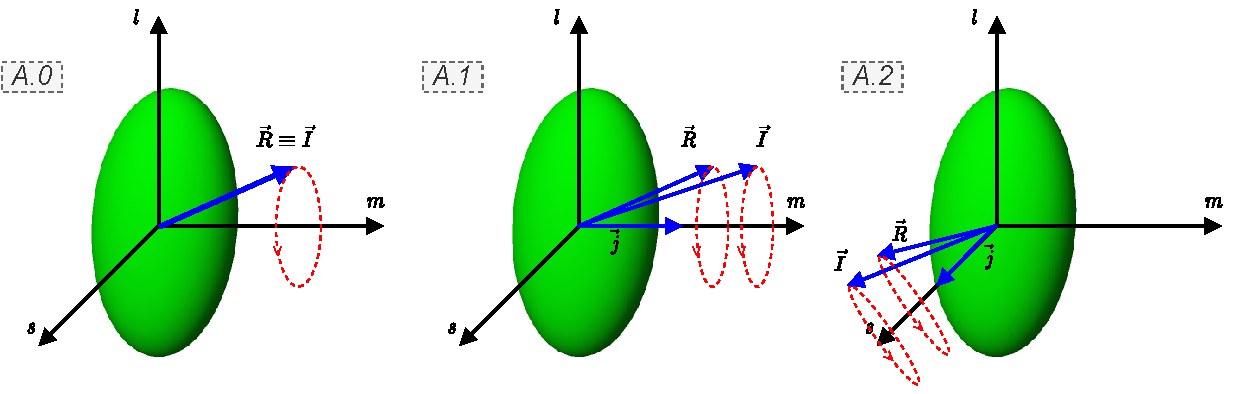
\includegraphics[width=0.95\textwidth]{figs/wobbling_Regimes_COUPLING_SCHEME.pdf}
    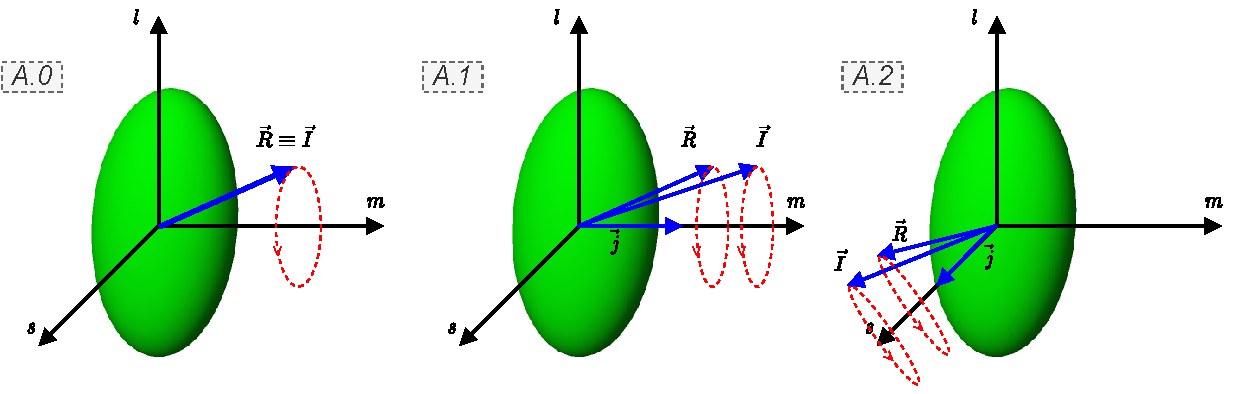
\includegraphics[scale=0.5]{figs/wobbling_Regimes_COUPLING_SCHEME.pdf}
    \caption{A.0: The geometry for the angular momentum of a simple wobbler. A.1: coupling geometry for a longitudinal wobbler (LW). A.2: coupling geometry for a transverse wobbler (TW). The short-$s$, long-$l$, and medium-$m$ axes are defined in the body-fixed frame. The vectors $\vec{R}$, $\vec{j}$, and $\vec{I}$ represent the set of angular momenta of the core, odd particle, and the total nuclear system, respectively.}
    \label{wobbling-coupling-scheme}
\end{figure}

The current work represents the second piece of a two-part series of papers that focuses on the description of the wobbling properties in odd-mass nuclei. Starting from an existing formalism concerning the interpretation of the wobbling structure of $^{163}$Lu \cite{raduta2020approach,raduta2020towards}, that initial framework (which will be further denoted by \texttt{W1}) is extended with a proper description of the states with positive and negative parity, by adopting the concept of \emph{Parity Partner Bands}. In the newly developed approach (denoted hereafter by \texttt{W2}), a single particle (the odd $i_{j=13/2}$ proton) couples to the triaxial core, generating a sequence of four triaxial strongly deformed bands (called $TSD_1$, $TSD_2$, $TSD_3$ and $TSD_4$), with a total of 63 rotational states in all the bands. Previously in \texttt{W1}, two different particle-core couplings were considered: one that consisted in the $i_{j=13/2}$ proton+core for the bands $TSD_{1,2,3}$ and one $h_{j=9/2}$ proton+core for $TSD_4$ band, which resulted in two separate fitting procedures required to obtain the energy spectrum of this isotope. Within \texttt{W2}, as per the first part of this series of papers (denoted throughout the paper with \textbf{I} \cite{poenaru2021parity}), a single fitting procedure was required to find the excitation energies of $^{163}$Lu, since only one proton was considered to align its angular momentum with that of the triaxial core. A successful description of the wobbling spectrum of $^{163}$Lu was made in \textbf{I}, together with calculation of other relevant quantities (e.g. rotational frequencies) that put \texttt{W2} to the test in terms of correctness. The obtained agreement with the experimental data was impressive.

In this second part (hereafter denoted by \textbf{II}), attention is given to the properties of the classical energy function of $^{163}$Lu, and the geometrical interpretation of the total angular momentum. The classical expression of the energy function, which can be obtained via the Time-Dependent Variational Principle (TDVE) applied in \textbf{I} allows the study of the wobbling stability, and also provides an insight into the classical features of nucleonic motion within the angular momentum space. Its expression signifies the initial quantal Hamiltonian of the deformed system but is brought to a dequantized form with the help of a set of coordinates that describe the dynamics. By expressing the angular momentum vector $I$ of the triaxial nucleus and the energy function $E$ as surfaces in a three-dimensional space, it is possible to obtain the trajectories of the rotating system by intersecting the two shapes. This aspect will be analyzed in detail later on.

The structure of this work is as follows. In Section 2 a brief overview of the key characteristics for the \texttt{W2} approach that emerged from \textbf{I} is made. In Section 3, the prerequisites for obtaining a classical expression of the energy function are formulated. Section 4 is devoted to the numerical results concerning the wobbling stability of $^{163}$Lu. Wobbling stability is studied in terms of contour plots of the aforementioned energy function. The nuclear trajectories (i.e., the intersection curves of the energy surface with angular momentum surface) of the system are graphically represented for given values of angular momentum and energy. Several regimes of rotational motion emerge from this analysis. Discussion of the results is also made in Section 4. The conclusions of this current work are given in Section 5.

\section{New formalism for the description of wobbling states}

The \texttt{W2} formalism which emerged in \textbf{I} \cite{poenaru2021parity} consists in a re-interpretation of the four wobbling bands from $^{163}$Lu. Namely, the bands $TSD_2$ and $TSD_4$ are \emph{parity partner bands}: $\Delta I=2$ sequences with identical spins but opposite parity ($\pi_{2}=+1$ and $\pi_{4}=-1$). Arguments for this came from the analysis of the wave function of the system. The function is an admixture of states with both positive and negative parity since the initial Hamiltonian is symmetric to rotations by a specific amount ($D_2$ implies invariance to rotations by $\pi$). A complete description of the properties of the wave function and the Hamiltonian concerning the parity property is made in \textbf{I}. In terms of wobbling excitations, both $TSD_2$ and $TSD_4$ are considered to be ground-state bands (zero-wobbling-phonon), obtained by coupling the $j_1=13/2$ proton (with parity $\pi_{j_1}=+1$) to a triaxial core of odd spins $R_2^+=1^+,3^+,5^+,\dots$ for $TSD_2$ and $R_2^-=1^-,3^-,5^-,\dots$ for $TSD_4$. The band $TSD_1$ is also regarded as as a ground state band, but here the proton couples to a core of even spin states $R_1=0^+,2^+,4^+,\dots$, and $TSD_3$ is indeed an excited wobbling band (one-wobbling-phonon) that is built on top of $TSD_2$ via the action of a phonon operator. The coupling schemes for \texttt{W2} are described in \textbf{I} (denoted by $C_1'$, $C_2'$, and $C_3'$). For a clearer picture, Appendix \ref{appendix:a} contains a diagram with all three mechanisms (see Fig. \ref{three-couplings}).

It is worth noting that this interpretation of the wobbling structure of $^{163}$Lu contrasts the previously known band configuration \cite{jensen2004coexisting,tanabe2006algebraic,frauendorf2014transverse} where the bands $TSD_2$ and $TSD_3$ were regarded as one- and two-wobbling phonon excitations built on the yrast $TSD_1$ band. However, it was recently shown \cite{raduta2020towards,raduta2020approach,raduta2020new} that $TSD_1$ and $TSD_2$ behave as signature partner bands, both being ground states with the favored (unfavored) $\alpha_f=+\frac{1}{2}$ ($\alpha_u=-\frac{1}{2}$) band as $TSD_1$ ($TSD_2$). This aspect, together with the fact that bands 2 and 4 are parity partners are the main ideas behind the \texttt{W2} formalism adopted in \textbf{I} and \textbf{II}. The workflow involved in \texttt{W2} is drawn in Fig. \ref{w2-model-worfklow}, and for the sake of completeness, the initial \texttt{W1} approach is also sketched in Fig. \ref{w1-model-worfklow} from Appendix \ref{appendix:a}.

\section{Theoretical Formalism}\label{section-theory}

In this section, a description of the framework used for obtaining the wobbling spectrum of $^{163}$Lu is made. As stated in the previous section, the system is described with a similar Hamiltonian used in \texttt{W1}, namely the Hamiltonian for the triaxial PRM.
\begin{align}
    H=H_\text{core}+H_\text{s.p.}\ .
    \label{prm-hamiltonian}
\end{align}

The Hamiltonian from Eq. \ref{prm-hamiltonian} describes a system in which an odd $j$ particle interacts with a triaxial even-even core i.e., the odd nucleon is moving in a quadrupole deformed mean-field that is generated by the core. As such, the first term in the Hamiltonian $H_\text{core}$ describes the motion of a triaxial core, while the second term $H_\text{s.p.}$ represents the single-particle potential characterizing the valence proton.

Indeed, the core Hamiltonian is given by:
\begin{align}
    H_\text{core}=\sum_{i=1,2,3}\frac{1}{2\mathcal{I}_i}(I_i-j_i)^2\ ,
    \label{core-hamiltonian}
\end{align}
where the core angular momentum is $\vec{R}=\vec{I}-\vec{j}$ and the terms $\mathcal{I}_i$ represent the moments of inertia for a triaxial ellipsoid, along the principal axes. These three moments of inertia will be considered as free parameters in the present calculations, but, compared to the work \texttt{W1}, a unique set of MOIs will be attributed to the four bands, since the triaxial core will create an alignment with a unique particle, that is $j_1$. Because of this, there is no option for their nature (i.e., rigid or hydrodynamic).

The single-particle Hamiltonian from Eq. \ref{prm-hamiltonian} is derived from the well-known Nilsson potential \cite{meyer1975collective,wang2008description}:
\begin{align}
    h(\beta_2,\gamma)=C\left\{\cos\gamma Y_{20}(\theta,\varphi)+\frac{\sin\gamma}{\sqrt{2}}\left[Y_{22}(\theta,\varphi)+Y_{2-2}(\theta,\varphi)\right]\right\}\ ,
    \label{nilsson-potential}
\end{align}
where the coupling parameter $C$ causes the level splitting in the deformed field and it is proportional to the quadrupole deformation $\beta_2$. The potential $h$ from Eq. \ref{nilsson-potential} is written in terms of the quadrupole deformation and triaxiality parameter that play the role of deformation parameters within a triaxial system $(\beta_2,\gamma)$. Its expression using the coupling parameter $C$ is widely used when working with a particle-rotor-model \cite{peng2003description,koike2004chiral,wang2007doublet}. In the present this case, the change $h(\beta_2,\gamma)\to H_\text{s.p.}$ is done by applying the Wigner-Eckart theorem for the single-$j$ particle, and the following expression for $H_\text{s.p.}$ will be obtained:
\begin{align}
    H_\text{s.p.}=\frac{V}{j(j+1)}\left[\cos\gamma(3j_3^2-\vec{j}^2)-\sqrt{3}\sin\gamma(j_1^2-j_2^2)\right]+\epsilon_j\ .
    \label{single-particle-hamiltonian}
\end{align}

This term describes the motion of an odd particle with angular momentum $j$ in a mean-field generated by a triaxial core, with a potential strength $V$ characterized by the quadrupole deformation ($V\propto\beta_2)$. In fact, the single-particle potential strength $V$ will be considered as the fourth free parameter within the calculations and its behavior will dictate the coupling of the $j$ particle with all four TSD bands. The term $\epsilon_j$ from Eq. \ref{single-particle-hamiltonian} represents the single-particle energy that corresponds to the odd $j$ proton from the $i$-orbital. One should not mix up the $j_1$ proton notation used throughout the paper with the components of the single-particle angular momentum from  Eq. \ref{single-particle-hamiltonian}.

Regarding the triaxial deformation $\gamma$ which enters in Eq. \ref{single-particle-hamiltonian}, its value will be considered as another free parameter of the current problem. In other words, having $V$ and $\gamma$ as free parameters means that the system will be described by its deformation parameters which will be obtained through a fitting procedure, keeping an agreement with the experimental data regarding the excitation energies of the rotational states belonging to $TSD_{1,2,3,4}$.

From Eqs. \ref{core-hamiltonian} and \ref{single-particle-hamiltonian}, the free parameter set can be obtained, hereafter denoted by $\mathcal{P}$. It comprises three moments of inertia, the single-particle potential strength, and the triaxial deformation. As such, $\mathcal{P}$ can be written as:
\begin{align}
    \mathcal{P}=\left[\mathcal{I}_1,\mathcal{I}_2,\mathcal{I}_3,V,\gamma\right]\ .
    \label{parameter-set}
\end{align}

Solving the problem of \texttt{W2} is equivalent to finding the eigenvalues of $H$ given in Eq. \ref{prm-hamiltonian}. In a similar approach as in \texttt{W1}, the eigenvalues of interest are obtained on the base of a semi-classical approach. Thus, the first step is to perform a de-quantization procedure on $H$ through a TDVE \cite{raduta2007semiclassical,budaca2018tilted,raduta2017semiclassical}:
\begin{align}
    \delta\int_0^t\bra{\Psi_{IjM}}H-i\frac{\partial}{\partial t'}\ket{\Psi_{IjM}}dt'=0\ .
    \label{tdve}
\end{align}

Working within a semi-classical approach allows one to keep close contact with the system's dynamics in terms of equations of motion for the generalized coordinates. The trial function from Eq. \ref{tdve} is carefully chosen as a product of two basis states comprising the states with total angular momentum $I$ and $j$, respectively:
\begin{align}
    \ket{\Psi_{IjM}}=\mathbf{N}e^{z\hat{I}_-}e^{s\hat{j}_-}\ket{IMI}\ket{jj}\ ,
    \label{trial-function}
\end{align}
where the operators $\hat{I}_-$ and $\hat{j}_-$ denote the lowering operators for the intrinsic angular momenta $\vec{I}$ and $\vec{j}$, respectively, and $\mathbf{N}$ plays the role of the normalization constant. One must remark the fact that the states $\ket{IMI}$ and $\ket{jj}$ from Eq. \ref{trial-function} are extremal states for the operators $(\hat{I}^2,\hat{I}_3)$ and $(\hat{j^2},\hat{j_3})$, respectively, and they correspond to the maximally allowed states for a given set of angular momenta $I$ and $j$. As an observation, the trial function is an admixture of components of definite $K$, which is consistent with the fact that for a triaxial nucleus, $K$ is not a good quantum number.

The variables $z$ and $s$ from Eq. \ref{trial-function} are complex functions of time, and they play the role of classical coordinates in the phase spaces that describe the motion of the core and the odd particle:
\begin{align}
    z=\rho e^{i\varphi}\ ,\ s=fe^{i\psi}\ .
    \label{complex-variable-set}
\end{align}

In order to obtain a set of classical equations in a Hamilton Canonical form, a new pair of variables are introduced: 
\begin{align}
    r=\frac{2I}{1+\rho^2}\ ,\ t=\frac{2j}{1+f^2}\ ,
\end{align}
where $r\in\left[0,2I\right]$ and $t\in\left[0,2j\right]$.Thus the equations of motion acquire the form:
\begin{align}
    \frac{\partial\mathcal{H}}{\partial r}&=\dot{\varphi}\ ;\ \frac{\partial\mathcal{H}}{\partial \varphi}=-\dot{r}\ , \nonumber\\
    \frac{\partial\mathcal{H}}{\partial t}&=\dot{\psi}\ ;\ \frac{\partial\mathcal{H}}{\partial \psi}=-\dot{t}\ .
    \label{eq-motion}
\end{align}

The function $\mathcal{H}$ denotes the average of the Hamiltonian operator $H$ (Eq. \ref{prm-hamiltonian}) with the trial function $\ket{\Psi_{IjM}}$ given in Eq. \ref{trial-function}, and it plays the role of classical energy:
\begin{align}
    \mathcal{H}(\varphi,r;\psi,t)=\bra{\Psi_{IjM}}H\ket{\Psi_{IjM}}\ ,
\end{align}

Starting from the equations of motion given in Eq. \ref{eq-motion}, one can observe that the function $\mathcal{H}$ is a constant of motion, that is $\dot{\mathcal{H}}\equiv0$. This equation will define a surface, a so-called equi-energy surface $\mathcal{H}=\text{const}$. It is worth mentioning the fact that such equality holds since the entire set of equations of motion emerged from a variational principle. The sign of the Hessian associated to this classical function will indicate its stationary points. Among them, some are minima. The critical points which are of interest for the present study are those obtained when the following ordering for the three moments of inertia holds: $\mathcal{I}_1>\mathcal{I}_2>\mathcal{I}_3$. There is no restriction on $\gamma$.

With a linearization procedure for the equations of motion around the minimum point  of $\mathcal{H}$, a dispersion equation will be obtained:
\begin{align}
    \Omega^4+B\Omega^2+C=0\ .
    \label{dispersion-eq}
\end{align}

The above equation describes a harmonic type of motion for the nuclear system, with the solutions to this algebraic equation as the \emph{wobbling frequencies} $\Omega$. The terms $B$ and $C$ are  functions of total angular momentum $I$, single-particle a.m. $j$, inertial parameters $A_k=1/(2\mathcal{I}_k)\ ,\ k=1,2,3$, single-particle potential strength $V$, and triaxiality parameter $\gamma$.  The $B$ term from Eq. \ref{dispersion-eq} has the expression \cite{raduta2020approach}:
\begin{align}
 -B=\left[(2I-1)(A_3-A_1)+2jA_1\right]\left[(2I-1)(A_2-A_1)+2jA_1\right]+8A_2A_3Ij+\text{T}_B^1\text{T}_B^2\ ,
 \label{b_term}
 \end{align}
 where the terms $\text{T}_B^1$ and $\text{T}_B^2$ are defined defined as:
 \begin{align}
 \text{T}_B^1&=\left[(2j-1)(A_3-A_1)+2IA_1+V\frac{2j-1}{j(j+1)}\sqrt{3}(\sqrt{3}\cos\gamma+\sin\gamma)\right]\ , \nonumber \\
 \text{T}_B^2&=\left[(2j-1)(A_2-A_1)+2IA_1+V\frac{2j-1}{j(j+1)}2\sqrt{3}\sin\gamma\right]\ .
 \label{b_term-plus}
\end{align}

Accordingly, the $C$ term from Eq. \ref{dispersion-eq} has the expression \cite{raduta2020approach}:
\begin{align}
    C=&\left\{\left[(2I-1)(A_3-A_1)+2jA_1\right]\text{T}_C^1
- 4IjA_3^2\right \} \nonumber\\
      &\times\left\{\left[(2I-1)(A_2-A_1)+2jA_1\right]\text{T}_C^2-4IjA_2^2\right\}\ ,
      \label{c_term}
\end{align}
where the terms $\text{T}_C^1$ and $\text{T}_C^2$ are defined defined as:
\begin{align}
    \text{T}_C^1&=\left[(2j-1)(A_3-A_1)+2IA_1+V\frac{2j-1}{j(j+1)}\sqrt{3}(\sqrt{3}\cos\gamma+\sin\gamma)\right]\ , \nonumber\\
    \text{T}_C^2&=\left[(2j-1)(A_2-A_1)+2IA_1+V\frac{2j-1}{j(j+1)}2\sqrt{3}\sin\gamma\right]\ . 
    \label{c_term-plus}
\end{align}

It can be seen that the terms which enter in $B$ and $C$, namely $(\text{T}_B^1,\text{T}_B^2)$ from Eq. \ref{b_term-plus} and $(\text{T}_C^1,\text{T}_C^2)$ from Eq. \ref{c_term-plus} correspond to the quadrupole deformation that causes the single-particle to move in the mean-field of the triaxial core. The terms also define the triaxiality that the nucleus achieves once the odd proton couples to the triaxial core, driving the system up to a large (and stable) deformation.

Going back to Eq. \ref{dispersion-eq}, under the restrictions for the MOIs defined above, the dispersion equation admits two real and positive solutions (hereafter denoted with $\Omega_1^I$ and $\Omega_2^I$, where $\Omega_1^I<\Omega_2^I$) defined for $j_1=i_{13/2}$, given by:
\begin{align}
    \Omega_{1,2}^I=\sqrt{\frac{1}{2}\left(-B\mp(B^2-4C)^{1/2}\right)}\ .
    \label{wobbling-frequencies}
\end{align}

These two solutions are interpreted as \emph{wobbling frequencies} associated with the motion of the core, and the motion of the odd-particle respectively. As such, each wobbling frequency has an associated wobbling-phonon number:
\begin{align}
    \Omega_1^I \to n_{w_1}\ ;\ \Omega_2^I \to n_{w_2}\ .
\end{align}


Now  the analytical expressions for the four TSD bands in $^{163}$Lu are readily obtained:
\begin{align}
    E_\text{TSD1}^I&=\epsilon_j+\mathcal{H}_\text{min}^{(I,j)}+\mathcal{F}_{00}^I\ ,\ I=13/2,17/2,21/2\dots \nonumber \\
    E_\text{TSD2}^I&=\epsilon_j^1+\mathcal{H}_\text{min}^{(I,j)}+\mathcal{F}_{00}^I\ ,\ I=27/2,31/2,35/2\dots \nonumber \\
    E_\text{TSD3}^I&=\epsilon_j+\mathcal{H}_\text{min}^{(I-1,j)}+\mathcal{F}_{10}^{I-1}\ ,\ I=33/2,37/2,41/2\dots \nonumber \\
    E_\text{TSD4}^I&=\epsilon_j^2+\mathcal{H}_\text{min}^{(I,j)}+\mathcal{F}_{00}^I\ ,\ I=47/2,51/2,55/2\dots\ ,
    \label{wobbling_energies}
\end{align}
where $\mathcal{F}_{n_{w_1}n_{w_2}}^I$ is a function of the wobbling frequencies:
\begin{align}
    \mathcal{F}_{n_{w_1}n_{w_2}}^I=\Omega_1^I\left(n_{w_1}+\frac{1}{2}\right)+\Omega_2^I\left(n_{w_2}+\frac{1}{2}\right)\ ,
    \label{f-term}
\end{align}
and $\mathcal{H}_\text{min}^{(I,j)}$ is the classical energy evaluated in its minimal point. For the present case, its analytical expression is given by the following equation:
\begin{align}
\mathcal{H}_\text{min}^{(I,j)}=(A_2+A_3)\frac{I+j}{2}+A_1(I-j)^2-V\frac{2j-1}{j+1}\sin\left(\gamma+\frac{\pi}{6}\right)\ .
    \label{hmin:equation}
\end{align}

A few aspects regarding the energy spectrum defined in Eq. \ref{wobbling_energies} are worth mentioning. To each band, there is a specific energy $\epsilon_j$ associated with the single-particle state. In this case, the odd-proton $j_1=13/2$ from the $i$-orbital is the one that couples to the triaxial core. However, for the bands $TSD_2$ and $TSD_4$, a different re-normalization of $\epsilon_j$ is considered, since $TSD_2$ is the unfavored signature partner of $TSD_1$, and $TSD_4$ is the negative parity partner of $TSD_2$ within the band structure. These quantities will shift the overall energy states belonging to the two bands, each by a different amount. As a result, both $\epsilon_j^1$ and $\epsilon_j^2$ will be adjusted throughout the numerical calculations such that the energy spectrum is best reproduced. Another aspect concerns the band $TSD_3$; since this is the only excited wobbling band within the family, its configuration is built on top of $TSD_2$, with the action of a single phonon ($n_{w_1}=1$) operator. Consequently, an energy state $I$ belonging to $TSD_3$ is obtained from a state $I-1$ from $TSD_2$.

\subsection{Energy function - geometrical interpretation}

The analytical expression for the average of $H$ with the trial function describing the system was previously calculated in \texttt{W1}. Indeed, the energy function $\mathcal{H}$ was given in terms of the phase space coordinates $(r,\varphi;t,\psi)$ as follows \cite{raduta2020approach}:
\begin{align}
    \mathcal{H}=&\frac{I}{2}(A_1+A_2)+A_3I^2+\frac{2I-1}{2I}r(2I-r)\mathcal{A}_\varphi+\frac{j}{2}(A_1+A_2)+A_3j^2+\frac{2j-1}{2j}t(2j-t)\mathcal{A}_\psi \nonumber\\
    &-2\sqrt{r(2I-r)t(2j-t)}\mathcal{A}_{\varphi\psi}+A_3\left[r(2j-t)+t(2I-r)\right]-2A_3Ij+V\frac{2j-1}{j+1}\mathcal{A}_\gamma\ ,
    \label{energy-function-analytical}
\end{align}
with:
\begin{align}
    &\mathcal{A}_\varphi(\varphi)=(A_1\cos^2\varphi+A_2\sin^2\varphi-A_3)\ , \nonumber\\
    &\mathcal{A}_{\varphi\psi}(\varphi,\psi)=(A_1\cos\varphi\cos\psi+A_2\sin\varphi\sin\psi)\ ,\nonumber\\
    &\mathcal{A}_\psi(\psi)=(A_1\cos^2\psi+A_2\sin^2\psi-A_3)\ , \nonumber\\
    &\mathcal{A}_\gamma(t,\psi)=\left[\cos\gamma-\frac{t(2j-t)}{2j^2}\sqrt{3}(\sqrt{3}\cos\gamma+\sin\gamma\cos2\psi)\right]\ .
\end{align}

It is instructive to check the dependence of the energy function on the angular momentum components, e.g., the coordinates $x_k\overset{\mathrm{not.}}{=}I_k\ ,\ k=1,2,3$, where the quantization axis is chosen as the 3-axis. By expressing the angular momentum coordinates $x_{1,2,3}$ in terms of the polar angles $(\theta,\varphi)$ and a radius $I$ , one obtains: 
\begin{align}
    x_1=I\sin\theta\cos\varphi\ ,\ x_2=I\sin\theta\sin\varphi\ ,\ x_3=I\cos\theta\ .
    \label{coordinate-parametrization}
\end{align}

Using this coordinates system and evaluating the energy function around its minimum point $p_0=(0,I;0,j)$, the following expression for $\mathcal{H}$ will be obtained:
\begin{align}
    %\left. \mathcal{H}\ \right\vert_{p_0}=I\left(I-\frac{1}{2}\right)\sin^2\theta(A_1\cos^2\varphi+A_2\sin^2\varphi-A_3)-2A_1Ij\sin\theta+T_\text{core}+T_\text{s.p.}\ .
    \left. \mathcal{H}\ \right\vert_{p_0}=I\left(I-\frac{1}{2}\right)\sin^2\theta\cdot\mathcal{A}_\varphi(\varphi)-2A_1Ij\sin\theta+T_\text{core}+T_\text{s.p.}\ .
    \label{energy-function-minimal}
\end{align}

The last two terms in this equation are independent on the polar angles $(\theta,\varphi)$ and they have the following form:
\begin{align}
    T_\text{core}&=\frac{I}{2}(A_1+A_2)+A_3I^2\ ,\nonumber \\
    T_\text{s.p.}&=\frac{j}{2}(A_2+A_3)+A_1j^2-V\frac{2j-1}{j+1}\sin\left(\gamma+\frac{\pi}{6}\right)\ .
    \label{energyfunction-core-single-particle-subterms}
\end{align}

The classical equations of motion admit two constants of motion: the total energy (E) and the total angular momentum (I).  Consequently, by finding the intersection line(s) between the energy surface $E$ and the surface of the angular momentum (i.e., a sphere of radius $r=I$), the system's trajectory at that particular energy and spin is obtained. Such representations will be made in the following section.

By changing Eq. \ref{energy-function-minimal} from polar coordinates into Cartesian coordinates, the energy surface $E$ will become:
\begin{align}
    E=&\left(1-\frac{1}{2I}\right)A_1x_1^2+\left(1-\frac{1}{2I}\right)A_2x_2^2+\left[\left(1-\frac{1}{2I}\right)A_3+A_1\frac{j}{I}\right]x_3^2-\nonumber\\
    &-I\left(I-\frac{1}{2}\right)A_3-2A_1Ij+T_\text{rot}+T_\text{sp}\ .
    \label{energy-ellipsoid-cartesian}
\end{align}

Indeed, one can notice that the three coordinates $x_k$ appear as a squared sum. If some notations for the terms appearing next to the coordinates and the free ones are made, one arrives at the following expression for the energy surface:
\begin{align}
    E=\mathcal{S}_1x_1^2+\mathcal{S}_2x_2^2+\mathcal{S}_3x_3^2+C_0^\text{rot+sp}\ .
    \label{energy-surface-short-expr}
\end{align}

From Eq. \ref{energy-surface-short-expr}, it is now clear that the energy surface will be an ellipsoid, while the free-term $\mathcal{C}_0^\text{rot+sp}$ will produce an overall shift of the entire surface. The shift is in fact caused by the core+particle coupling.

 For a total angular momentum $\vec{I}$, the vector generates a sphere of radius $r=I$ described by the equation:
\begin{align}
    I^2=x_1^2+x_2^2+x_3^2\ .
    \label{angular-momentum-sphere}
\end{align}

The trajectories obtained through the intersection of Eqs. \ref{energy-ellipsoid-cartesian} and \ref{angular-momentum-sphere} will show a classical visualization of the wobbling character for a triaxial nucleus.

\section{Numerical results}
\label{section-results}

The resulting values for $\mathcal{P}$ are given  in Table \ref{parameter_set}. This \texttt{W2} method contrasts the approach in \texttt{W1}, where a second minimization process was needed separately for $TSD_4$. The root mean square error provided by the obtained parameter set $\mathcal{P}$ has a value of $E_\text{rms}\approx 79\ \text{keV}$. This result is much better than the one obtained with previous formalism \texttt{W1} where an $E_\text{rms}\approx240\ \text{keV}$ was obtained \cite{raduta2020approach}). As a matter of fact, this is the first semi-classical formalism in the literature that achieves agreement with the experimental data with less than $100\ \text{keV}$ for the entire wobbling spectrum of $^{163}$Lu. It is worth mentioning that the fitting procedure was done not for the absolute wobbling energies $E_\text{TSDk}^I\ ,\ k=1,2,3,4$, but for the \emph{excitation energies} which are relative to the hand-head $I=13/2^+$ from the first yrast band $TSD_1$.

\begin{table}
\caption{The parameter set $\mathcal{P}$ that was determined by a fitting procedure of the excitation energies for $^{163}$Lu.}
    \centering
  \begin{tabular}{lllll}
  \hline
$\mathcal{I}_1$ [$\hbar^2$/\text{MeV}] & $\mathcal{I}_2$ [$\hbar^2$/\text{MeV}]& $\mathcal{I}_3$ [$\hbar^2$/\text{MeV}] & $\gamma$ [deg. ] & $V$ [\text{MeV}] \\
\hline
\hline
72              & 15              & 7               & 22       & 2.1\\
\hline
\end{tabular}
    \label{parameter_set}
\end{table}

\subsection{Stability of the wobbling region}\label{wobbling-stability}

The expression for the classical energy function, which plays a crucial role in analyzing the nucleus's stability for a given rotational state, was presented in the previous section, through Eq. \ref{energy-function-minimal}. This will be used within the present numerical calculations to pinpoint the regions in space where the minimal points of $\mathcal{H}$ do exist. A special interest is devoted to the low-lying states from each of the four bands. Namely, for each band, a spin-state close to the band-head is chosen, then using the parameter set $\mathcal{P}$, a graphical representation in the $(\theta,\varphi)$-coordinate space is realized, and in each case, the extremal points with minimum character are identified. These graphical representations are shown in Figures \ref{contours-12} and \ref{contours-34}.

\begin{figure}
\centering
\begin{minipage}{.5\textwidth}
  \centering
  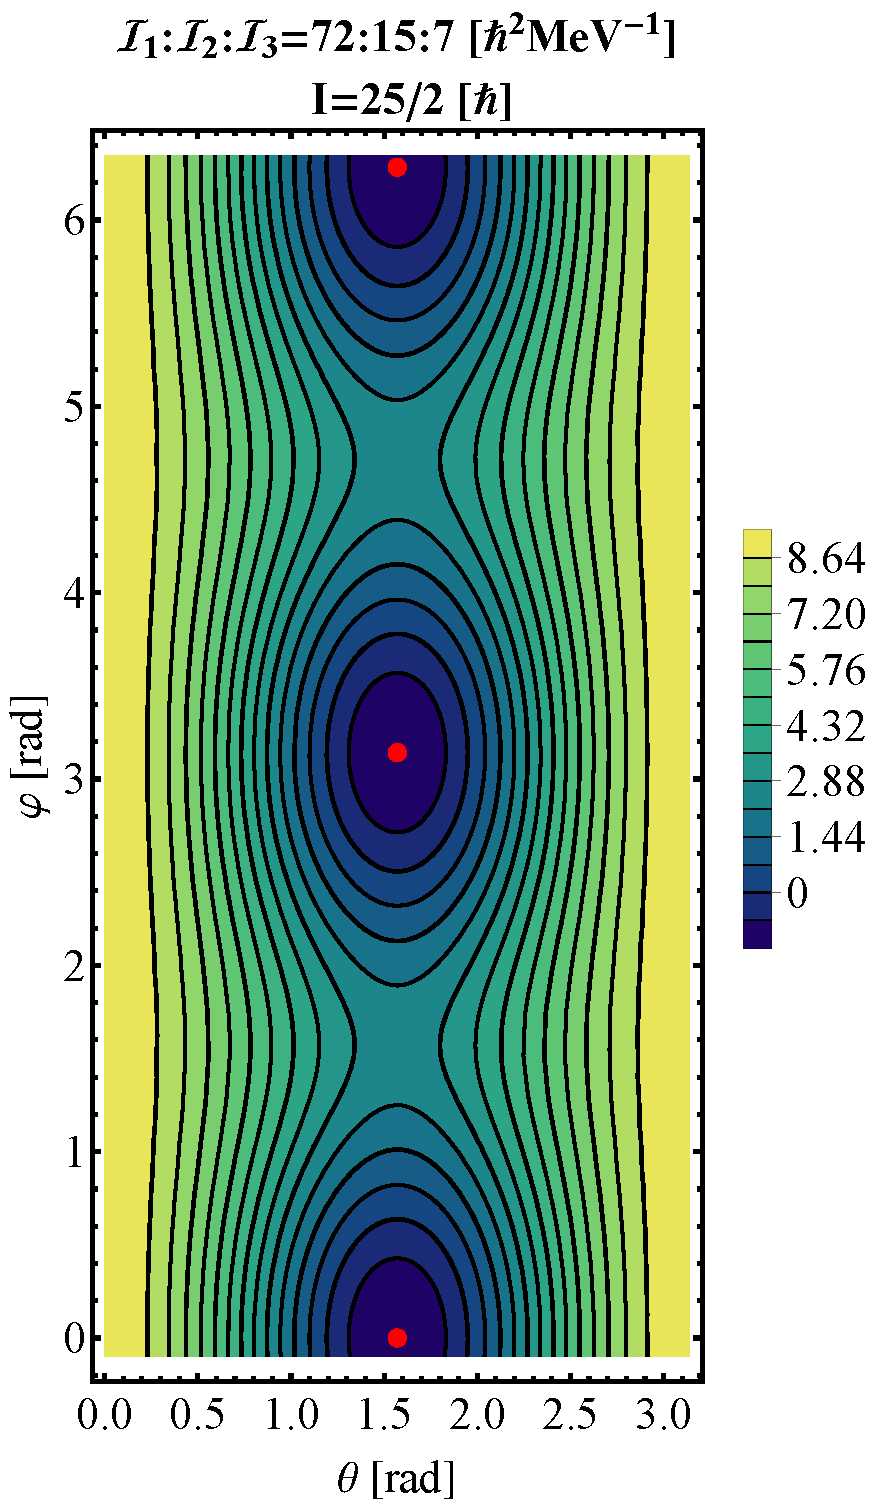
\includegraphics[scale=0.2]{figs/contour-tsd1.pdf}
\end{minipage}%
\begin{minipage}{.5\textwidth}
  \centering
 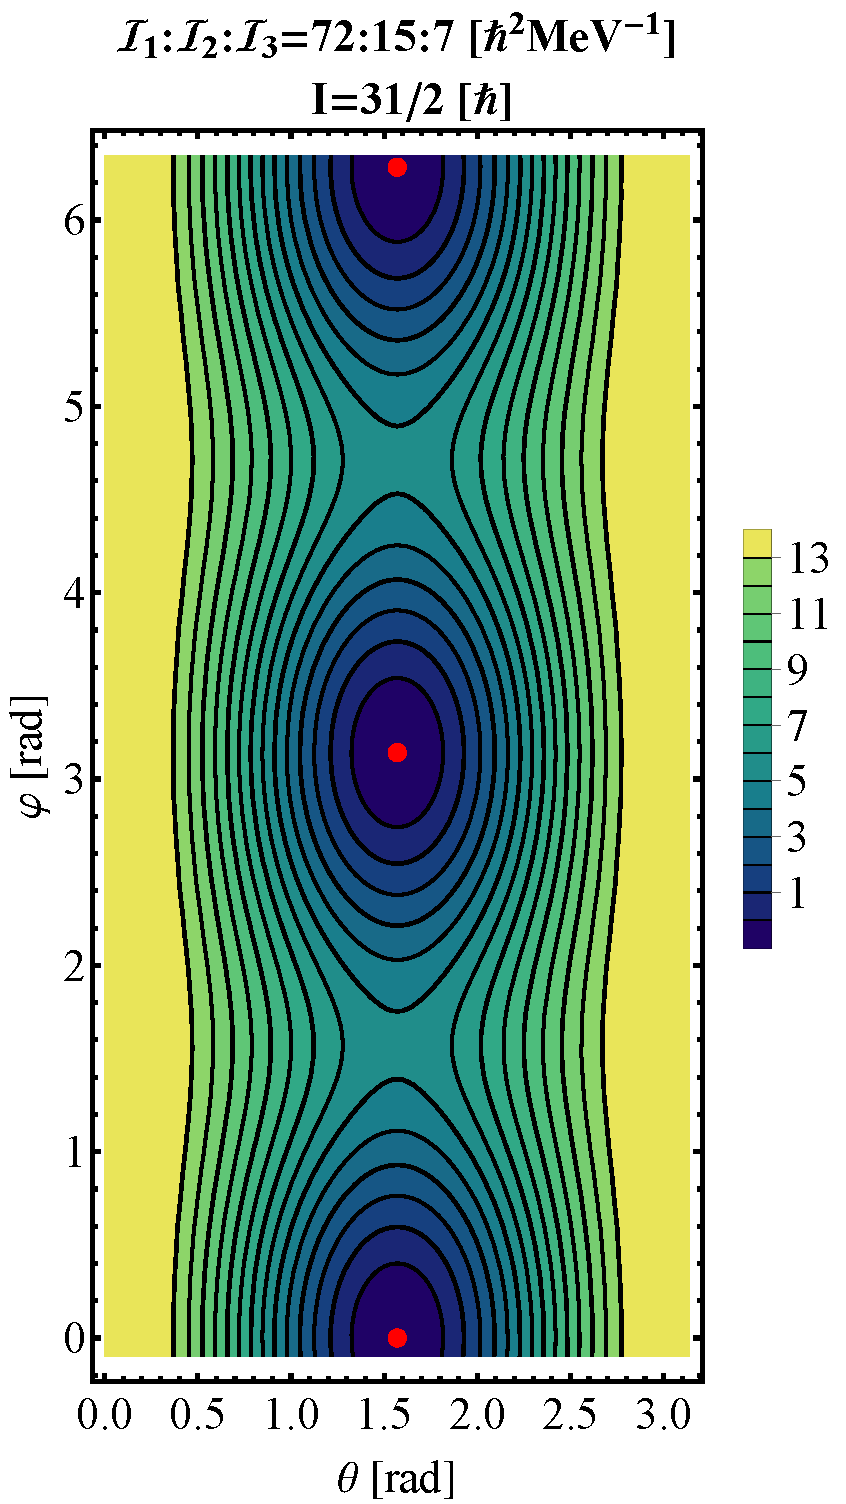
\includegraphics[scale=0.2]{figs/contour-tsd2.pdf}
\end{minipage}
\caption{Contour plots with the energy function $\mathcal{H}$ given by Eq. \ref{energy-function-minimal} for a state in $TSD_1$ (left) and a state from $TSD_2$ (right). Calculations were performed with the numerical parameters given in Table \ref{parameter_set}. The minimum points for $\mathcal{H}$ are marked by red dots, and they represent the regions in space where the nucleus has a stable wobbling character. The darker \emph{islands} also indicate a stable motion of the triaxial nucleus.}
    \label{contours-12}
\end{figure}

The four contour plots shown in Figures \ref{contours-12} and \ref{contours-34} have many similarities, suggesting common collective properties, but also differences which are caused by the fact that the minima have different depths. A common feature consists in that the equi-energy curves surround a sole minimum for low values in energy, but as the energy increases, the trajectories go around all minima, the lack of localization indicating unstable wobbling motion. The unstable regions might also relate to phase transitions, where the nucleus can undergo a major change in its rotational character. This aspect will also be discussed in the next subsection, devoted to the 3-dimensional representation of the energy ellipsoid and the classical trajectories of the triaxial system.

\begin{figure}
\centering
\begin{minipage}{.5\textwidth}
  \centering
  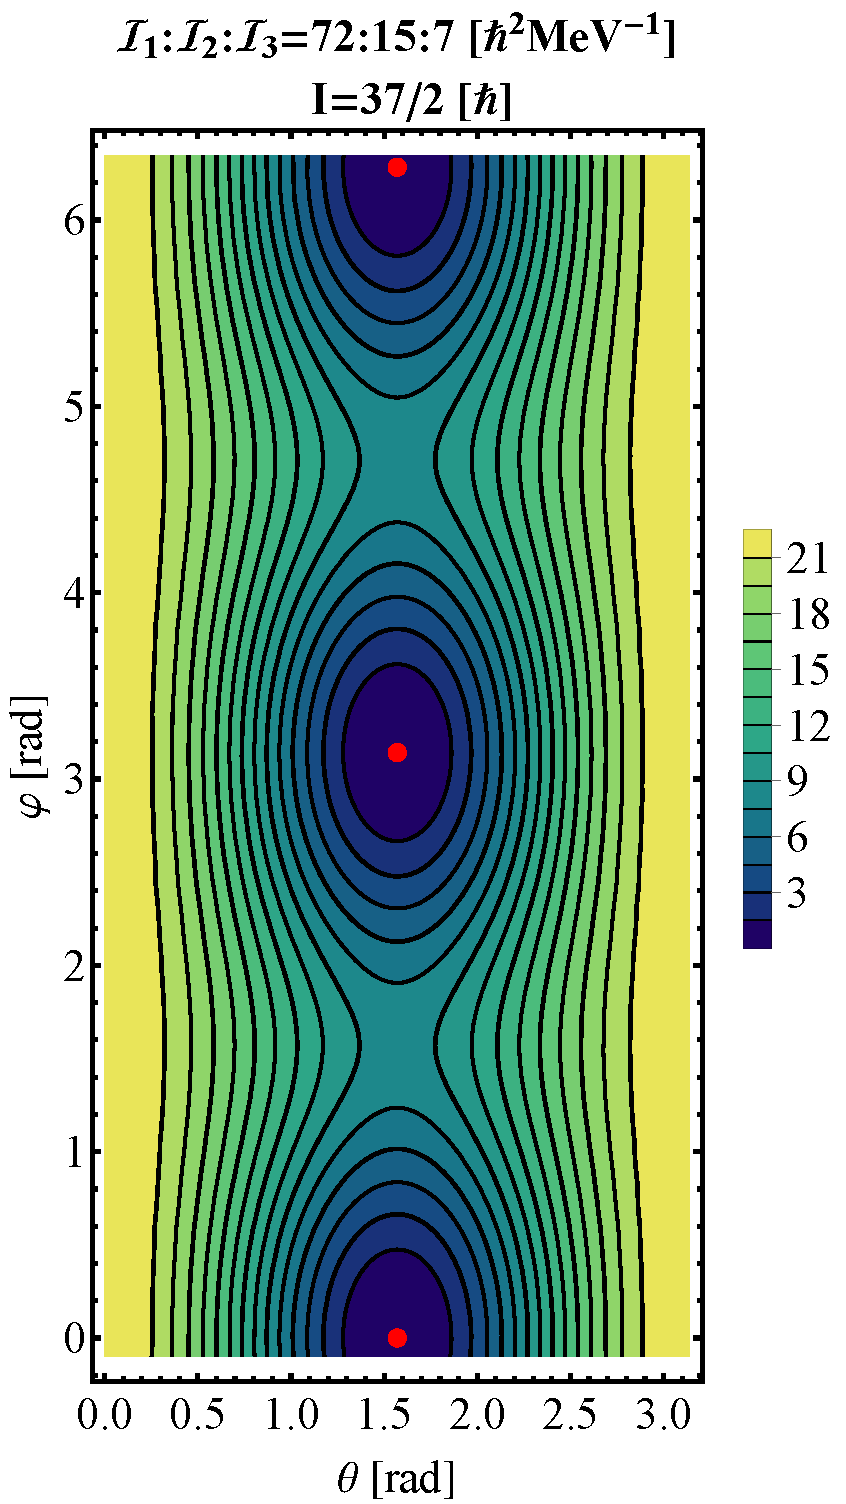
\includegraphics[scale=0.2]{figs/contour-tsd3.pdf}
\end{minipage}%
\begin{minipage}{.5\textwidth}
  \centering
 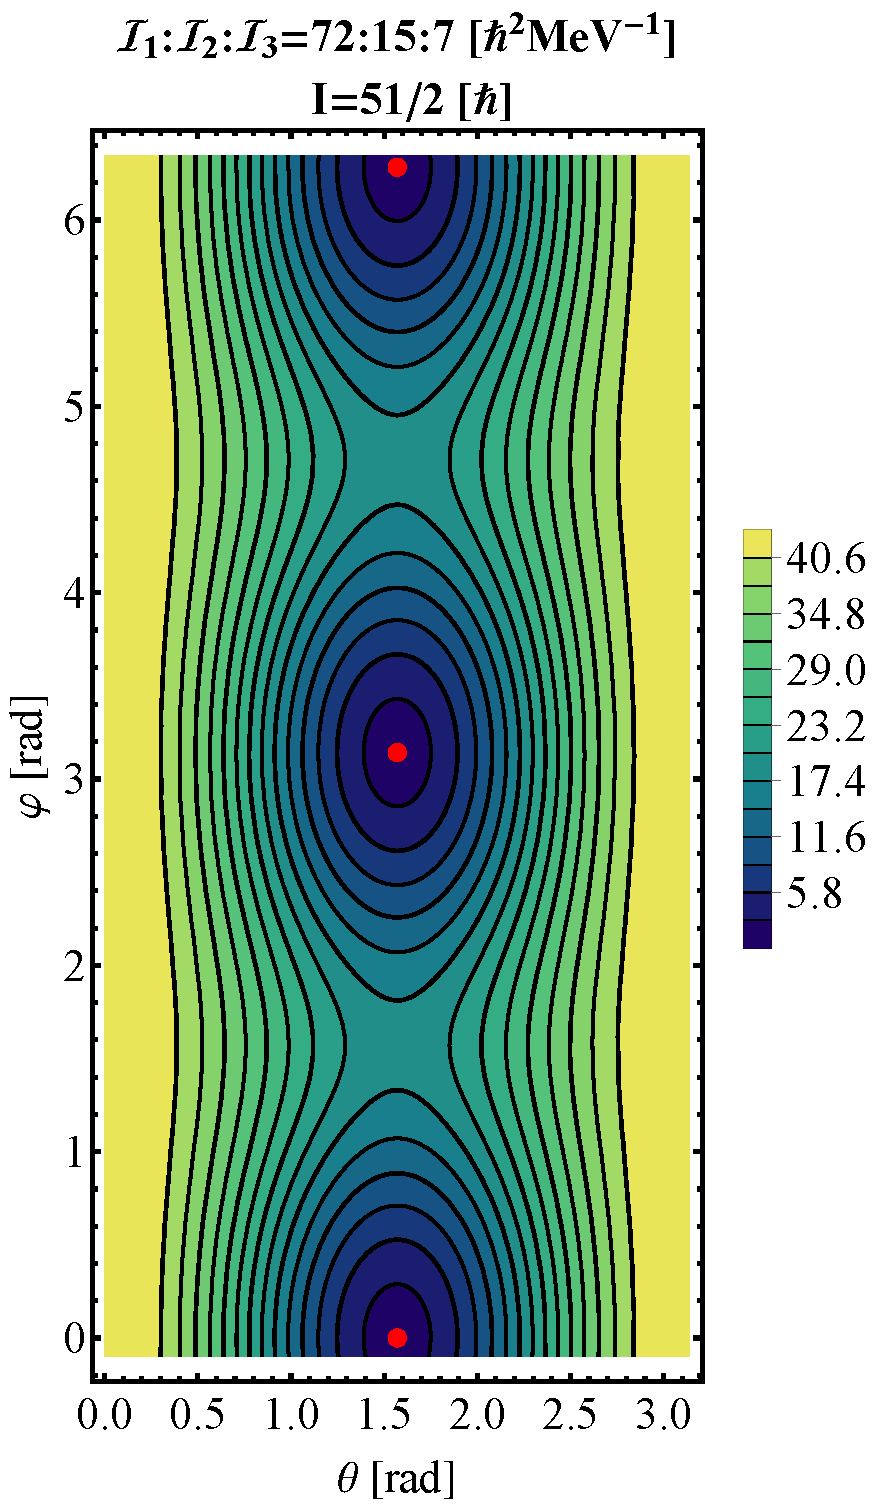
\includegraphics[scale=0.2]{figs/contour-tsd4.pdf}
\end{minipage}
\caption{Contour plots with the energy function $\mathcal{H}$ given by Eq. \ref{energy-function-minimal} for a state in $TSD_3$ (left) and a state from $TSD_4$ (right). Calculations were performed with the numerical parameters given in Table \ref{parameter_set}. The minimum points for $\mathcal{H}$ are marked by red dots, and they represent the regions in space where the nucleus has a stable wobbling character. The darker \emph{islands} also indicate a stable motion of the triaxial nucleus.}
    \label{contours-34}
\end{figure}

Regarding the minimum points (marked by red dots on the contour plots), their position remains unchanged for all four bands and any rotational state $I$, as long as the MOI order stays the same. Remarkable is the fact that only with the obtained set of parameters (i.e., the current MOI ordering) it was possible to define contours with stable motion (marked by the darker regions). Indeed, if the two ratios $\mathcal{I}_1/\mathcal{I}_2$ and $\mathcal{I}_2/\mathcal{I}_3$ would have been smaller, a larger unstable region would prevail (with islands of maximal character), constraining thus the stable wobbling motion. This could indicate the fact that the single-particle term $T_\text{s.p.}$ from $\mathcal{H}$ is sensitive to larger triaxiality, and only for certain values will the system achieve a stable motion characterized by large deformation (see Eq. \ref{energyfunction-core-single-particle-subterms}).

An additional step consists in the analysis of the energy function, more precisely to see its evolution in one of the minimum points with respect to the angular momentum $I$. As it was already observed from the contour plots shown in Figures \ref{contours-12}-\ref{contours-34}, the depth of the minima differs from one spin state to another, so it would be useful to have a quantitative view on that change. By fixing $\mathcal{H}$ in one of its critical points (e.g., the minimum $p_\text{min}(\theta,\varphi)=(\frac{\pi}{2},0)$), the angular momentum $I$ was varied within a large interval, and the evolution of $\mathcal{H}$ was evaluated. Graphical representation is shown in Figure \ref{energy-function-minimum-evolution}.

\begin{figure}
    \centering
    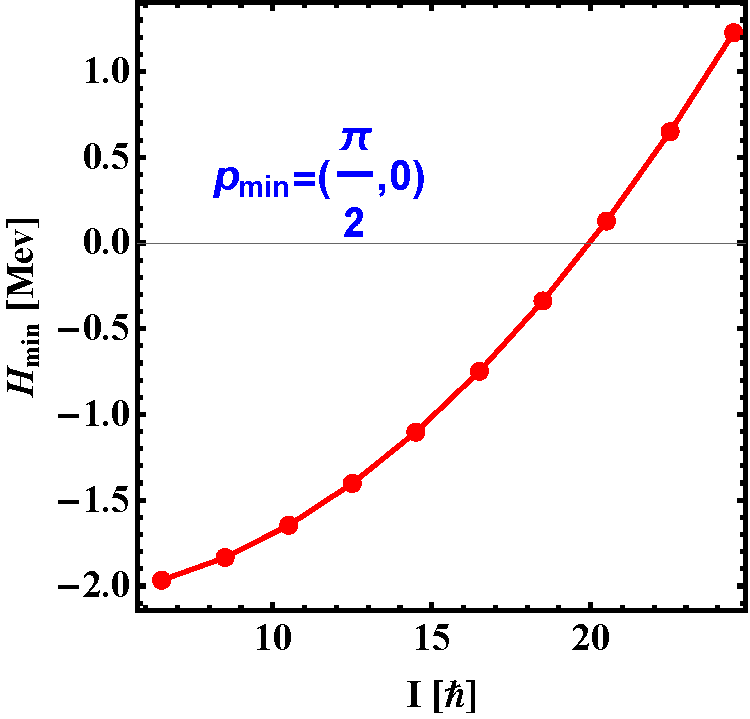
\includegraphics[scale=0.50]{figs/energy_function_minPoint_Evolution.pdf}
    \caption{The change in the minimum depth of $\mathcal{H}$, evaluated in the one of its critical points $p_\text{min}(\theta,\varphi)=(\frac{\pi}{2},0)$, using the parameters given in Table \ref{parameter_set}.}
    \label{energy-function-minimum-evolution}
\end{figure}

As it can be seen from Figure \ref{energy-function-minimum-evolution}, the classical energy $\mathcal{H}$ is an increasing function of angular momentum, which is to be expected, since the wobbling energies of the four bands increase with respect to the increase in spin. The negative values of $\mathcal{H}$ for low-lying wobbling states do not indicate that the nucleus has negative energy states since \emph{the rest} of the nucleus' energy is also given by the single-particle energy $\epsilon_j$ terms and the phononic $\mathcal{F}_{n_{w_1}n_{w_2}}^I$ terms.

Another useful insight would be the study of the classical energy function $\mathcal{H}$ as a function of the polar angles $(\theta,\varphi)$. This can be achieved by choosing a minimum point, keeping one of the polar coordinates fixed, and then let the other one vary across its corresponding interval. For $^{163}$Lu, such a graphical representation was done for the point $p_\text{min}=\left(\frac{\pi}{2},0\right)$ (that is the bottom-most red dot from each of the four contour plots depicted in Figures \ref{contours-12}-\ref{contours-34}). Results can be seen in Figure \ref{energy-function-min-point-evolution}.

\begin{figure}
\centering
\begin{minipage}{.5\textwidth}
  \centering
  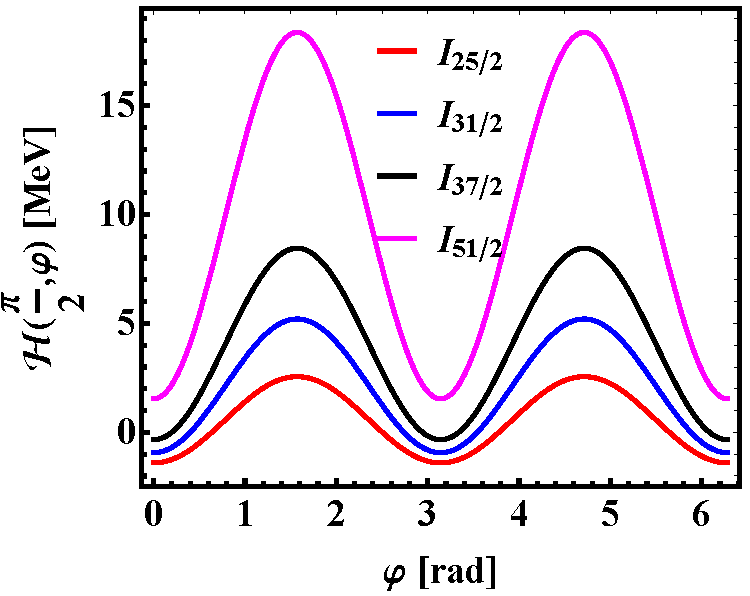
\includegraphics[scale=0.48]{figs/energyFunction_minTheta.pdf}
\end{minipage}%
\begin{minipage}{.5\textwidth}
  \centering
 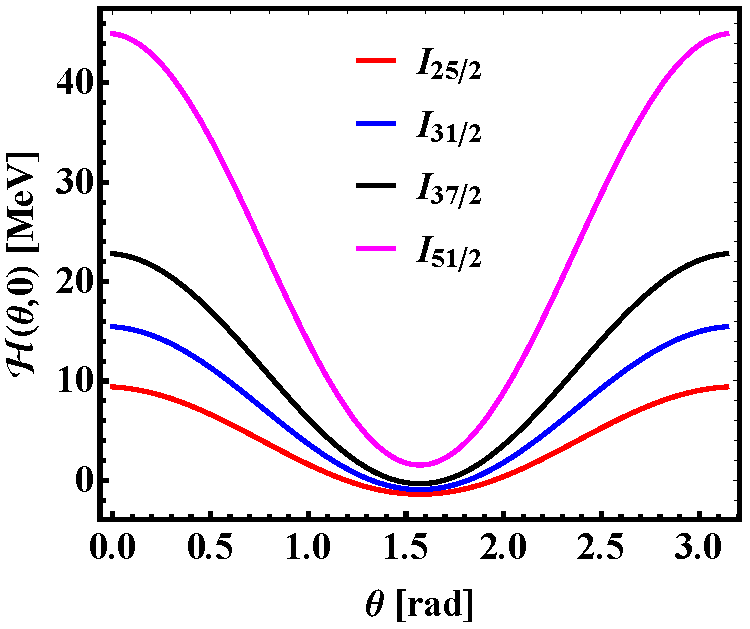
\includegraphics[scale=0.45]{figs/energyFunction_minVarphi.pdf}
\end{minipage}
\caption{The energy function $\mathcal{H}$, evaluated in one of its minimum points, as a function of the polar coordinates. One coordinate is fixed while the other one is varied within its interval of existence. For $\theta\in[0,\pi]$ and $\varphi\in[0,2\pi]$. The chosen minimum is $p_\text{min}=\left(\frac{\pi}{2},0\right)$. Each spin state corresponds to one of the four triaxial bands of $^{163}$Lu (with $I_{25/2}\in TSD_1$, $I_{31/2}\in TSD_2$, $I_{37/2}\in TSD_3$, and $I_{51/2}\in TSD_4$).}
    \label{energy-function-min-point-evolution}
\end{figure}


\subsection{Classical trajectories - 3D representation}\label{classical-trajectories}

The final step of the present work is to obtain an insight into the classical features of $^{163}$Lu concerning the total angular momentum and its rotational motion. As already mentioned, the trajectories are given by the intersection curves of the energy ellipsoid $E$ given in Eq. \ref{energy-ellipsoid-cartesian} with the angular momentum sphere $I$ given in Eq. \ref{angular-momentum-sphere}. In the 3-dimensional space generated by the three components of the angular momentum vector $\vec{I}$, these intersection curves characterize the motion of the system, as each curve will be oriented along with one of the three axes $x_k\ ,\ k=1,2,3$, suggesting a rotational motion (the precession of the total a.m.) around a particular direction preferred by the system.

As such, the dependence of the classical trajectories on the angular momenta as well as on energies must be analyzed in $\texttt{W2}$. Indeed, when the model Hamiltonian is diagonalized for a given $I$, a set of $2I+1$ energies are obtained. Therefore, it is justified to study the evolution of trajectories when the energy of the nucleus is increasing. The curves are represented as the manifold given by the intersection of the two constants of motion, that is $E$ and $I$. An example of such trajectories are depicted in Figures \ref{trajectories-12}-\ref{trajectories-34}.

\begin{figure}
    \centering
    % 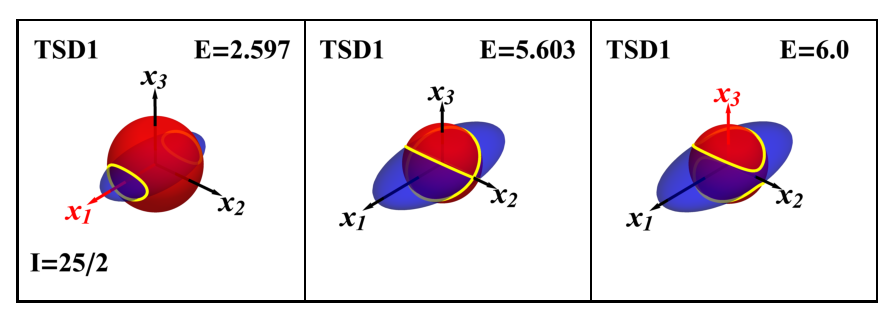
\includegraphics[width=0.8\textwidth]{figs/tsd1_spin1.eps}
    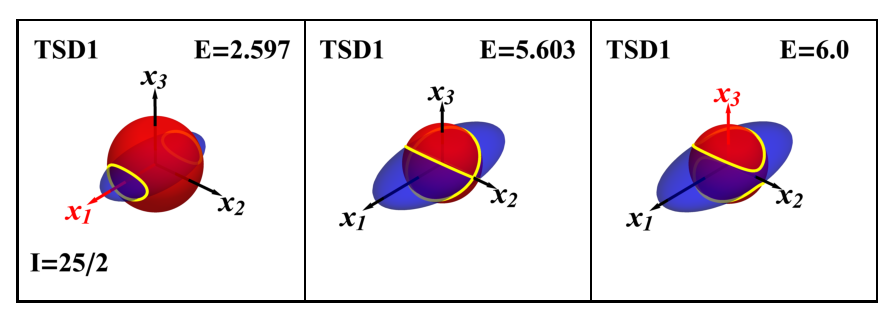
\includegraphics[scale=0.7]{figs/tsd1_spin1.eps}
    % 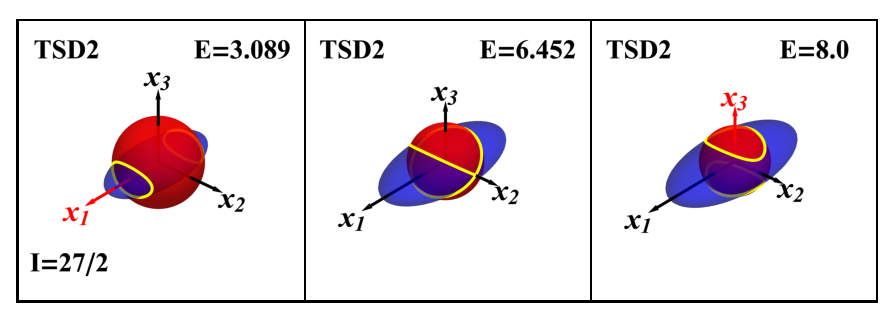
\includegraphics[width=0.8\textwidth]{figs/tsd2_spin1.eps}
    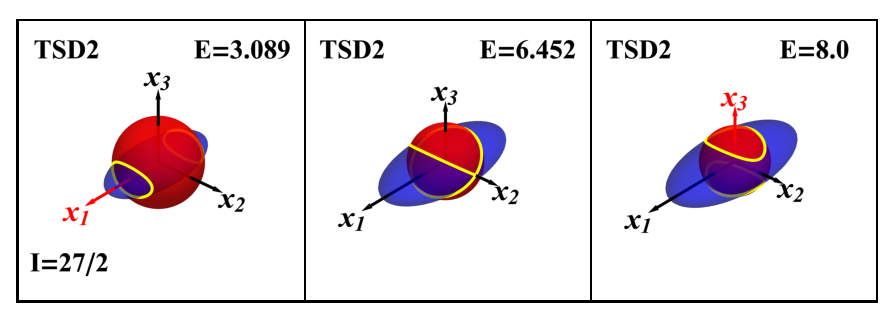
\includegraphics[scale=0.7]{figs/tsd2_spin1.eps}
    \caption{The nuclear trajectories of the system, evaluated for two spin states belonging to $TSD_1$ and $TSD_2$. Intersection lines marked by yellow color represents the actual orbits. Axis colored in red represents the direction along which the system rotates (it precesses). The left-most inset corresponds to the real excitation energy for that particular spin state $I$.}
    \label{trajectories-12}
\end{figure}


\begin{figure}
    \centering
    % 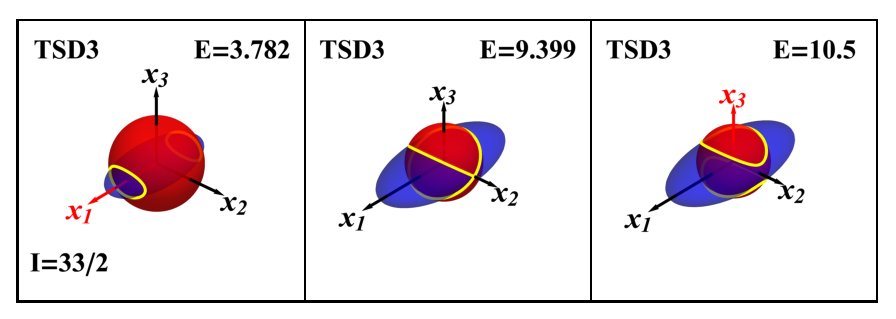
\includegraphics[width=0.8\textwidth]{figs/tsd3_spin1.eps}
    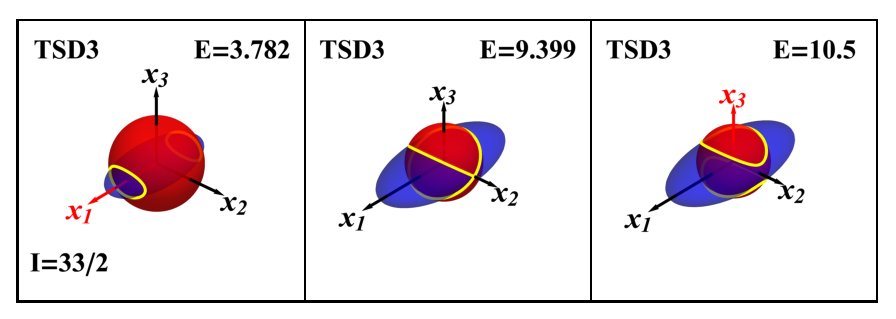
\includegraphics[scale=0.7]{figs/tsd3_spin1.eps}
    % 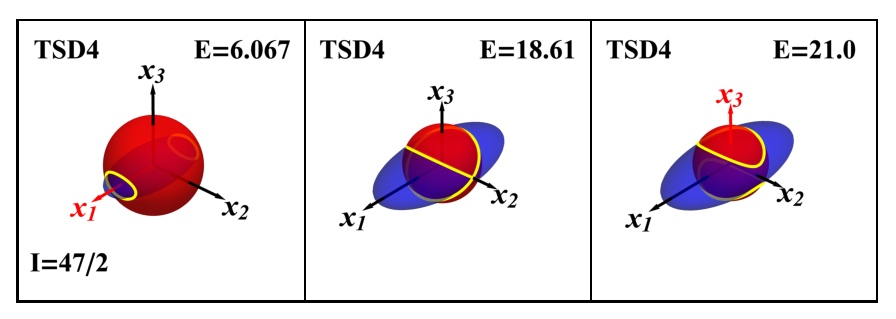
\includegraphics[width=0.8\textwidth]{figs/tsd4_spin1.eps}
    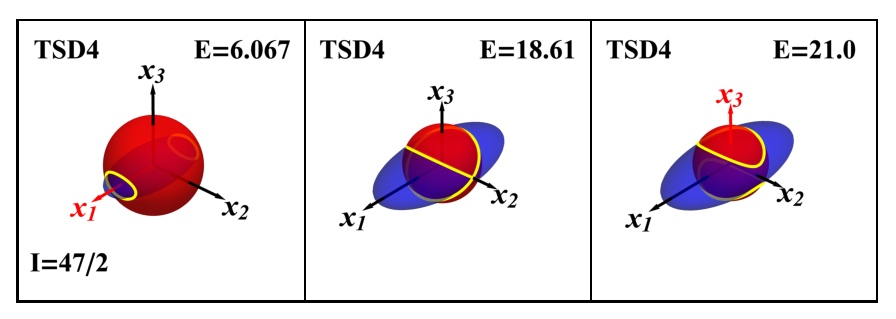
\includegraphics[scale=0.7]{figs/tsd4_spin1.eps}
    \caption{The nuclear trajectories of the system, evaluated for two spin states belonging to $TSD_3$ and $TSD_4$. Intersection lines marked by yellow color represents the actual orbits. Axis colored in red represents the direction along which the system rotates (it precesses). The left-most inset corresponds to the real excitation energy for that particular spin state $I$.}
    \label{trajectories-34}
\end{figure}

Each row from the Figures \ref{trajectories-12}-\ref{trajectories-34} represents a rotational state within a band. A low-lying spin state was chosen from each band in particular as an example. The left inset of each row represents the real excitation energy for the state $I$ at which the energy ellipsoid is evaluated. It can be seen that two distinct (but symmetric) trajectories are observed along the 1-axis, for all four states. This suggests that the states of the triaxial nucleus are obtained from the rotation of the angular momentum along $x_1$. Indeed, for low energies, the rotation is more pronounced along the $x_1$- and $-x_1$-axes. As the energy of the nucleus increases, the two trajectories approach each other, which results in a tilted rotation axis corresponding to both curves. The tilted axis implies that the rotation axis is being misaligned, the rotational axis moving away from its \emph{equilibrium point}, marking the tilted-axis-rotation. Note that this picture is fully consistent with the one described by Lawrie et al. \cite{lawrie2020tilted}. Further increase in energy will result in the two trajectories intersect with each other. The point where the intersection between the two orbits occurs is marked in the middle inset from each figure. Consequently, the intersection of these two orbits marks an unstable motion within the system. Finally, when the energy increases even more, beyond this \emph{critical point}, one arrives again in a two-trajectories regime but with a different rotation axis, lying closer to the $x_3$ axis. This case is shown in the right inset within each figure, where the axis $x_3$ is marked by red color, signaling the change in the rotational mode of the nucleus. However, it is worth noting that such energies are way too large for such a phase transition to occur naturally in $^{163}$Lu. For example, in the case of $I_{25/2}\in TSD_1$, the energy at which $^{163}$Lu undergoes a phase transition with regards to the rotational mode is close to $5.6\ \text{MeV}$ (middle inset for $TSD_1$ from Figure \ref{contours-12}), but the real excitation energy which corresponds to this state is half that value (left inset for $TSD_1$ from Figure \ref{trajectories-12}). Nevertheless, it is a remarkable fact that with the current model, a phase transition between rotational modes in a triaxial nucleus can be identified. A proper microscopic formalism based on this approach might also provide a more detailed picture with regards to the allowed trajectories for the system.

\section{Conclusions \& Outlook}
\label{section-gata}

Concluding the present work, this newly developed formalism proves to be a successful tool for accurately describing the wobbling spectrum of $^{163}$Lu and also for providing an insight into the rotational motion of the nuclear system with respect to its total spin.

\begin{acknowledgement}
This work was supported by UEFISCU, through the project \textbf{PCE-16/2021}.
\end{acknowledgement}

\appendix
\section{Appendix - Workflow Diagrams}
\label{appendix:a}
The two models described throughout the paper, namely the formalisms $\texttt{W1}$ and \texttt{W2} are schematically represented. The \texttt{W1} model corresponds to the work given in Refs. \cite{raduta2020approach,raduta2020towards}, and the \texttt{W2} corresponds to the formalism developed in this two-part series of papers. For \texttt{W1}, the diagram is shown in Figure \ref{w1-model-worfklow}, while for the newly developed approach \texttt{W2}, the diagram is shown in Figure \ref{w2-model-worfklow}. The coupling scheme for \texttt{W2} is also represented in Figure \ref{three-couplings}.

\begin{figure}
    \centering
    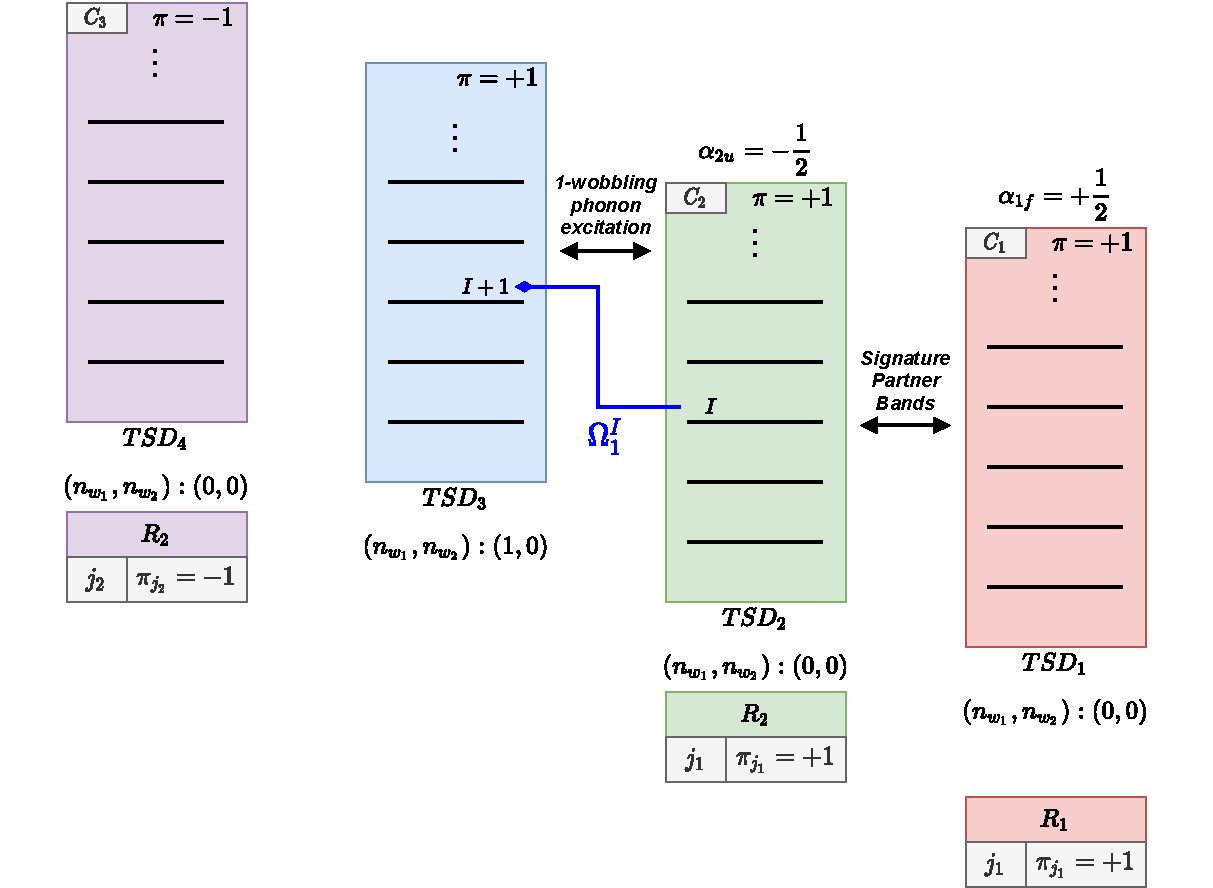
\includegraphics[width=0.95\textwidth]{figs/W1_Approach.pdf}
    \caption{Schematic representation of the band structure adopted for $^{163}$Lu in the \texttt{W1} model. For each band, the wobbling phonon numbers are shown. The main features and linking properties between bands are represented with arrows. The bottom part shows the coupling scheme (the core and the valence nucleon) for each wobbling band. The blue arrow marks the activation of $TSD_3$ states via the phonon operator.}
    \label{w1-model-worfklow}
\end{figure}
\begin{figure}
  \centering
    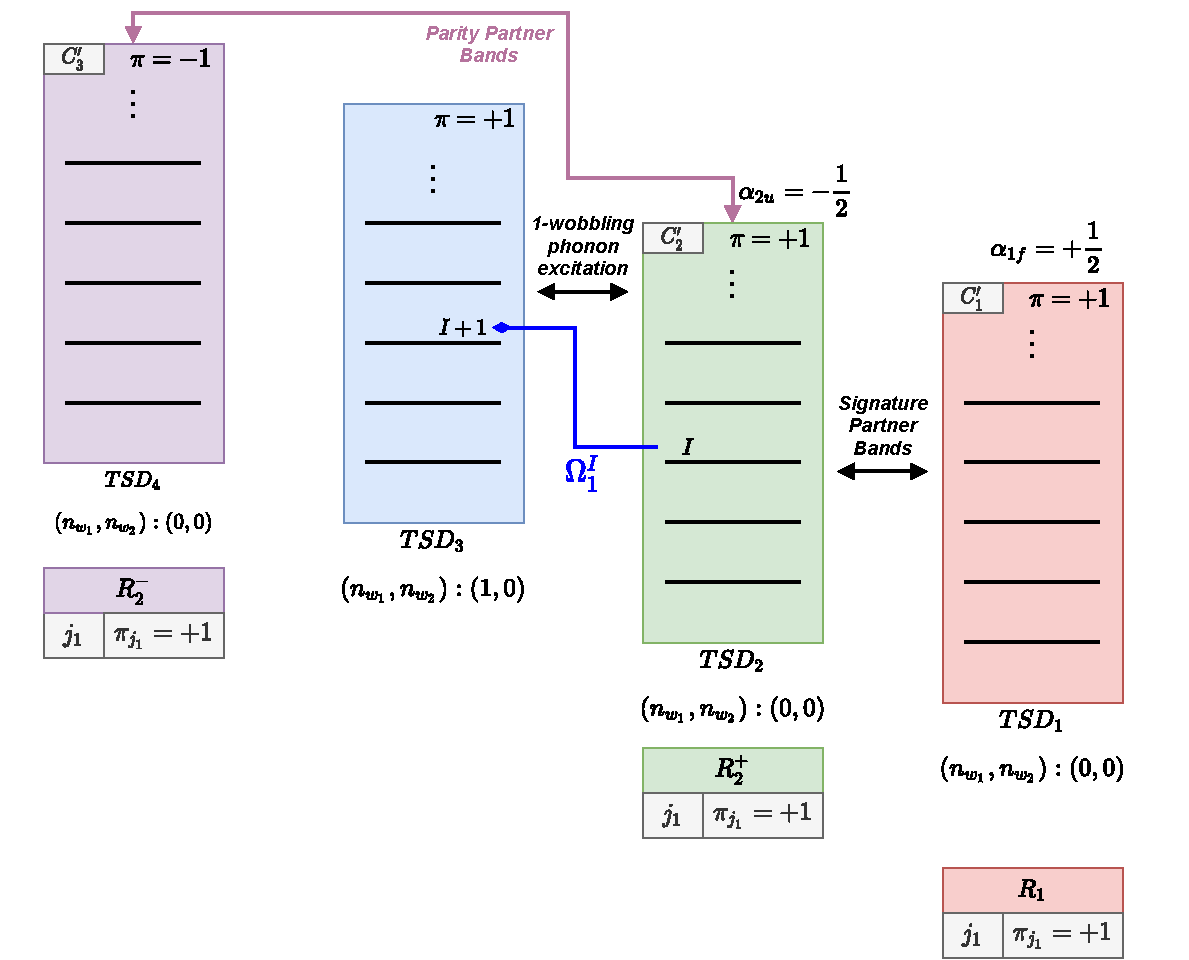
\includegraphics[width=0.95\textwidth]{figs/W2_Approach.pdf}
    \caption{Schematic representation of the band structure adopted for $^{163}$Lu in the \texttt{W2} model. For each band, the wobbling phonon numbers are shown. The main features and linking properties between bands are represented with arrows. The bottom part shows the coupling scheme (the core and the valence nucleon) for each wobbling band. The blue arrow marks the activation of $TSD_3$ states via the phonon operator.}
    \label{w2-model-worfklow}
\end{figure}
\begin{figure}
    \centering
    % 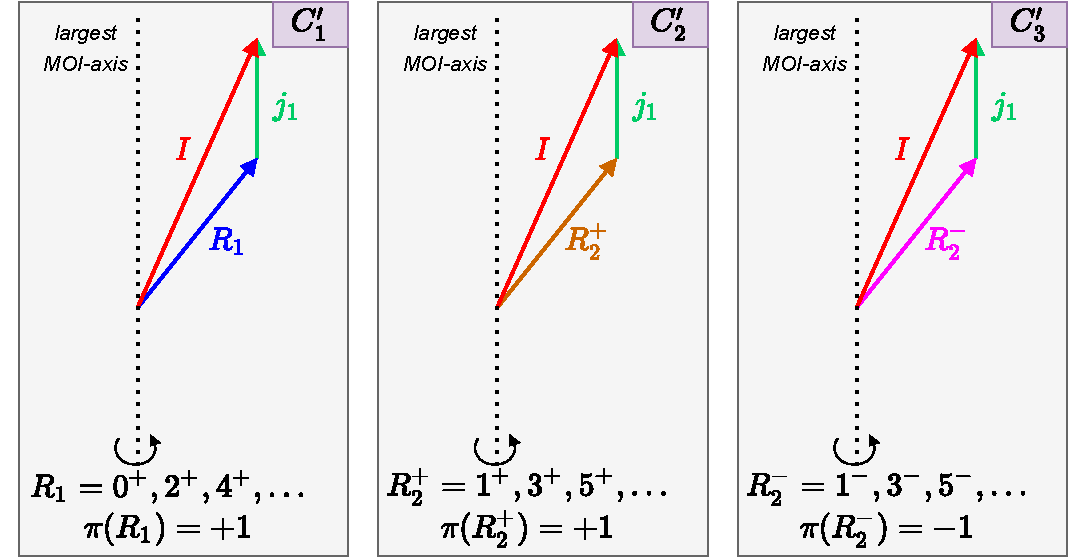
\includegraphics[width=0.95\textwidth]{figs/coupling_schemes_C1C2C3.pdf}
    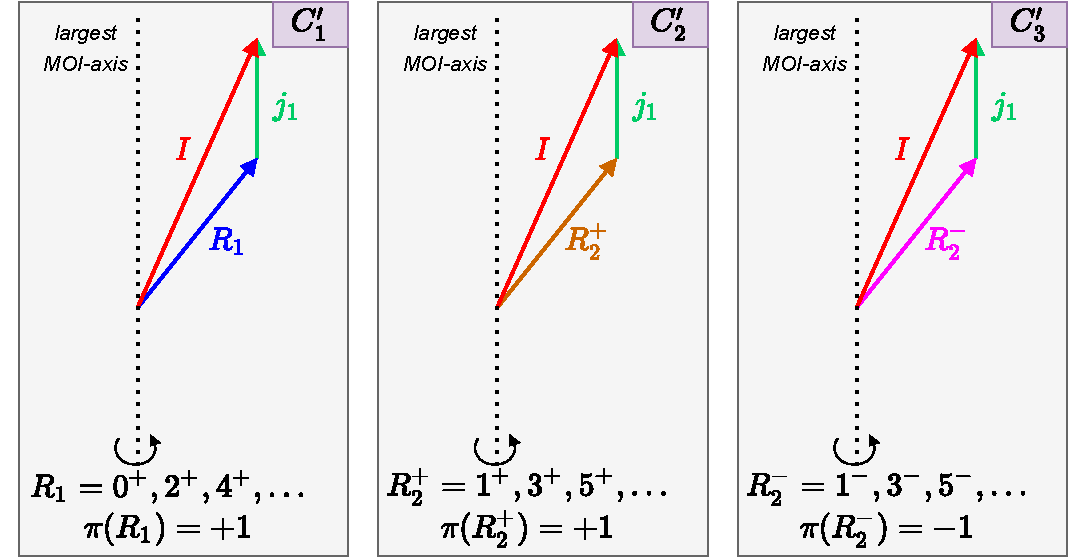
\includegraphics[scale=0.55]{figs/coupling_schemes_C1C2C3.pdf}
    \caption{A schematic representation with the three coupling schemes that characterize the \texttt{W2} model. The same odd particle ($j_1=i_{13/2}$ proton) is coupled with two positive cores with even (odd) integer spin sequences for $TSD_1$ ($TSD_2$), and one negative core in the case of $TSD_4$ with odd integer spin sequence. The total spin of the system precesses around the axis with the largest MOI, as it is the case for a triaxial rotor.}
    \label{three-couplings}
\end{figure}

\begin{thebibliography}{99}

\bibitem{moller2006global}
Peter M{\"o}ller, Ragnar Bengtsson, B~Gillis Carlsson, Peter Olivius, and
  Takatoshi Ichikawa.
\newblock{\em Physical review letters}, 97(16):162502, 2006.

\bibitem{moller2009heavy}
Peter M{\"o}ller, Arnold~J Sierk, Takatoshi Ichikawa, Akira Iwamoto, Ragnar
  Bengtsson, Henrik Uhrenholt, and Sven {\AA}berg.
\newblock{\em Physical Review C}, 79(6):064304, 2009.

\bibitem{hamamoto1988triaxial}
I~Hamamoto and H~Sagawa.
\newblock{\em Physics Letters B}, 201(4):415--419, 1988.

\bibitem{bengtsson1984signature}
R~Bengtsson, H~Frisk, FR~May, and JA~Pinston.
\newblock{\em Nuclear Physics A}, 415(2):189--214, 1984.

\bibitem{stachel1982triaxiality}
J~Stachel, N~Kaffrell, E~Grosse, H~Emling, H~Folger, R~Kulessa, and D~Schwalm.
\newblock{\em Nuclear Physics A}, 383(3):429--467, 1982.

\bibitem{frauendorf1997tilted}
Stefan Frauendorf and Jie Meng.
\newblock{\em Nuclear Physics A}, 617(2):131--147, 1997.

\bibitem{bohr1998nuclear}
Aage~Niels Bohr and Ben~R Mottelson.
\newblock{\em Nuclear Structure (In 2 Volumes)}.

\bibitem{bringel2005evidence}
P~Bringel, GB~Hagemann, H~H{\"u}bel, A~Al-Khatib, P~Bednarczyk, A~B{\"u}rger,
  D~Curien, G~Gangopadhyay, B~Herskind, DR~Jensen, et~al.
\newblock {\em The European Physical Journal A-Hadrons and Nuclei},
  24(2):167--172, 2005.

\bibitem{hartley2009wobbling}
DJ~Hartley, RVF Janssens, LL~Riedinger, MA~Riley, A~Aguilar, MP~Carpenter,
  CJ~Chiara, P~Chowdhury, IG~Darby, U~Garg, et~al.
\newblock {\em Physical Review C}, 80(4):041304, 2009.

\bibitem{amro2003wobbling}
H~Amro, WC~Ma, GB~Hagemann, RM~Diamond, J~Domscheit, P~Fallon, A~G{\"o}rgen,
  B~Herskind, H~H{\"u}bel, DR~Jensen, et~al.
\newblock {\em Physics Letters B}, 553(3-4):197--203, 2003.

\bibitem{schonwasser2003one}
G~Sch{\"o}nwa{\ss}er, H~H{\"u}bel, GB~Hagemann, P~Bednarczyk, G~Benzoni,
  A~Bracco, P~Bringel, R~Chapman, D~Curien, J~Domscheit, et~al.
\newblock {\em Physics Letters B}, 552(1-2):9--16, 2003.


\bibitem{xiong2019nuclear}
BW~Xiong and YY~Wang.
\newblock{\em Atomic Data and Nuclear Data Tables}, 125:193--225, 2019.

\bibitem{dimitrov2000chirality}
VI~Dimitrov, S~Frauendorf, and F~D{\"o}nau.
\newblock{\em Physical review letters}, 84(25):5732, 2000.

\bibitem{koike2003systematic}
T~Koike, K~Starosta, CJ~Chiara, DB~Fossan, and DR~LaFosse.
\newblock{\em Physical Review C}, 67(4):044319, 2003.

\bibitem{meng2006possible}
J~Meng, J~Peng, SQ~Zhang, and S-G Zhou.
\newblock{\em Physical Review C}, 73(3):037303, 2006.

\bibitem{raduta2016new}
AA~Raduta, Al~H Raduta, and CM~Petrache.
\newblock{\em Journal of Physics G: Nuclear and Particle Physics},
  43(9):095107, 2016.

\bibitem{petrache2018evidence}
CM~Petrache, BF~Lv, A~Astier, E~Dupont, YK~Wang, SQ~Zhang, PW~Zhao, ZX~Ren,
  J~Meng, PT~Greenlees, et~al.
\newblock{\em Physical Review C}, 97(4):041304, 2018.

\bibitem{lv2019chirality}
BF~Lv, CM~Petrache, QB~Chen, J~Meng, A~Astier, E~Dupont, P~Greenlees, H~Badran,
  T~Calverley, DM~Cox, et~al.
\newblock{\em Physical Review C}, 100(2):024314, 2019.

\bibitem{raduta2020towards}
AA~Raduta, R~Poenaru, and CM~Raduta.
\newblock{\em Journal of Physics G: Nuclear and Particle Physics},
  47(2):025101, 2020.
  
  \bibitem{poenaru2021parity}
R~Poenaru and AA~Raduta,
\newblock{\em Romanian Journal of Physics},
  Paper submitted, 2021.

\bibitem{hagemann2003quantized}
Gudrun~B Hagemann and Ikuko Hamamoto.
\newblock{\em Nuclear Physics News}, 13(3):20--24, 2003.

\bibitem{odegaard2001evidence}
SW~{\O}deg{\aa}rd, GB~Hagemann, DR~Jensen, M~Bergstr{\"o}m, B~Herskind,
  G~Sletten, S~T{\"o}rm{\"a}nen, JN~Wilson, PO~Tj{\o}m, I~Hamamoto, et~al.
\newblock{\em Physical review letters}, 86(26):5866, 2001.

\bibitem{jensen2002evidence}
DR~Jensen, GB~Hagemann, I~Hamamoto, SW~{\O}deg{\aa}rd, B~Herskind, G~Sletten,
  JN~Wilson, K~Spohr, H~H{\"u}bel, P~Bringel, et~al.
\newblock{\em Physical review letters}, 89(14):142503, 2002.

\bibitem{jensen2002wobbling}
D~Ringk{\o}bing Jensen, GB~Hagemann, I~Hamamoto, SW~{\O}deg{\aa}rd,
  M~Bergstr{\"o}m, B~Herskind, G~Sletten, S~T{\"o}rm{\"a}nen, JN~Wilson,
  PO~Tj{\o}m, et~al.
\newblock{\em Nuclear Physics A}, 703(1-2):3--44, 2002.

\bibitem{schnack1995superdeformed}
H~Schnack-Petersen, Ragnar Bengtsson, RA~Bark, P~Bosetti, A~Brockstedt,
  H~Carlsson, LP~Ekstr{\"o}m, GB~Hagemann, B~Herskind, F~Ingebretsen, et~al.
\newblock{\em Nuclear Physics A}, 594(2):175--202, 1995.

\bibitem{biswas2019longitudinal}
S~Biswas, R~Palit, S~Frauendorf, U~Garg, W~Li, GH~Bhat, JA~Sheikh, J~Sethi,
  S~Saha, Purnima Singh, et~al.
\newblock{\em The European Physical Journal A}, 55(9):1--7, 2019.

\bibitem{matta2017transverse}
James~Till Matta.
\newblock Transverse wobbling in 135 pr.
\newblock In {\em Exotic Nuclear Excitations: The Transverse Wobbling Mode in
  135 Pr}, pages 77--93. Springer, 2017.


\bibitem{sensharma2019two}
N~Sensharma, U~Garg, S~Zhu, AD~Ayangeakaa, S~Frauendorf, W~Li, GH~Bhat,
  JA~Sheikh, MP~Carpenter, QB~Chen, et~al.
\newblock{\em Physics Letters B}, 792:170--174, 2019.

\bibitem{chakraborty2020multiphonon}
S~Chakraborty, HP~Sharma, SS~Tiwary, C~Majumder, AK~Gupta, P~Banerjee,
  S~Ganguly, S~Rai, S~Kumar, A~Kumar, et~al.
\newblock{\em Physics Letters B}, 811:135854, 2020.

\bibitem{petrache_2018}
C~M Petrache.
\newblock{\em LNL Annual Report}, 2018.

\bibitem{timar2019experimental}
J~Tim{\'a}r, QB~Chen, B~Kruzsicz, D~Sohler, I~Kuti, SQ~Zhang, J~Meng, P~Joshi,
  R~Wadsworth, K~Starosta, et~al.
\newblock{\em Physical review letters}, 122(6):062501, 2019.

\bibitem{nandi2020first}
S~Nandi, G~Mukherjee, QB~Chen, S~Frauendorf, R~Banik, Soumik Bhattacharya,
  Shabir Dar, S~Bhattacharyya, C~Bhattacharya, S~Chatterjee, et~al.
\newblock{\em Physical Review Letters}, 125(13):132501, 2020.

\bibitem{sensharma2020longitudinal}
N~Sensharma, U~Garg, QB~Chen, S~Frauendorf, DP~Burdette, JL~Cozzi, KB~Howard,
  S~Zhu, MP~Carpenter, P~Copp, et~al.
\newblock{\em Physical review letters}, 124(5):052501, 2020.

\bibitem{guo2020risk}
S~Guo, XH~Zhou, CM~Petrache, EA~Lawrie, S~Mthembu, YD~Fang, HY~Wu, HL~Wang,
  HY~Meng, GS~Li, et~al.
\newblock{\em arXiv preprint arXiv:2011.14354}, 2020.

\bibitem{hamilton2010super}
JH~Hamilton, SJ~Zhu, YX~Luo, AV~Ramayya, S~Frauendorf, JO~Rasmussen, JK~Hwang,
  SH~Liu, GM~Ter-Akopian, AV~Daniel, et~al.
\newblock{\em Nuclear Physics A}, 834(1-4):28c--31c, 2010.

\bibitem{luo2013triaxial}
YX~Luo, JH~Hamilton, AV~Ramaya, JK~Hwang, SH~Liu, JO~Rasmussen, S~Frauendorf,
  GM~Ter-Akopian, AV~Daniel, Yu~Ts Oganessian, et~al.
\newblock Triaxial and triaxial softness in neutron rich ru and pd nuclei.
\newblock In {\em Exotic Nuclei: EXON-2012}, pages 215--224. World Scientific,
  2013.
  
\bibitem{petrache2019diversity}
CM~Petrache, PM~Walker, S~Guo, QB~Chen, S~Frauendorf, YX~Liu, RA~Wyss,
  D~Mengoni, YH~Qiang, A~Astier, et~al.
\newblock{\em Physics Letters B}, 795:241--247, 2019.

\bibitem{wang2020two}
YK~Wang, FQ~Chen, and PW~Zhao.
\newblock{\em Physics Letters B}, 802:135246, 2020.

\bibitem{chen2019transverse}
QB~Chen, S~Frauendorf, and CM~Petrache.
\newblock{\em Physical Review C}, 100(6):061301, 2019.

\bibitem{frauendorf2014transverse}
S~Frauendorf and F~D{\"o}nau.
\newblock{\em Physical Review C}, 89(1):014322, 2014.

\bibitem{hamamoto2002wobbling}
Ikuko Hamamoto.
\newblock{\em Physical Review C}, 65(4):044305, 2002.

\bibitem{tanabe2006algebraic}
Kosai Tanabe and Kazuko Sugawara-Tanabe.
\newblock{\em Physical Review C}, 73(3):034305, 2006.

\bibitem{wen2015wobbling}
Shi Wen-Xian and Chen Qi-Bo.
\newblock{\em Chinese Physics C}, 39(5):054105, 2015.

\bibitem{davydov1958rotational}
AS~Davydov and GF~Filippov.
\newblock{\em Nuclear Physics}, 8:237--249, 1958.

\bibitem{shimizu1995nuclear}
Yoshifumi~R Shimizu and Masayuki Matsuzaki.
\newblock{\em Nuclear Physics A}, 588(3):559--596, 1995.

\bibitem{matsuzaki2002wobbling}
Masayuki Matsuzaki, Yoshifumi~R Shimizu, and Kenichi Matsuyanagi.
\newblock{\em Physical Review C}, 65(4):041303, 2002.

\bibitem{matsuzaki2003dynamical}
Masayuki Matsuzaki, Yoshifumi~R Shimizu, and Kenichi Matsuyanagi.
\newblock{\em The European Physical Journal A-Hadrons and Nuclei},
  20(1):189--190, 2003.

\bibitem{matsuzaki2004instability}
Masayuki Matsuzaki and Shin-Ichi Ohtsubo.
\newblock{\em Physical Review C}, 69(6):064317, 2004.

\bibitem{matsuzaki2004nuclear}
Masayuki Matsuzaki, Yoshifumi~R Shimizu, and Kenichi Matsuyanagi.
\newblock{\em Physical Review C}, 69(3):034325, 2004.

\bibitem{shimizu2005high}
Yoshifumi~R Shimizu, Masayuki Matsuzaki, and Kenichi Matsuyanagi.
\newblock{\em Physical Review C}, 72(1):014306, 2005.

\bibitem{shimizu2008parametrizations}
Yoshifumi~R Shimizu, Takuya Shoji, and Masayuki Matsuzaki.
\newblock{\em Physical Review C}, 77(2):024319, 2008.

\bibitem{shoji2009microscopic}
Takuya Shoji and Yoshifumi~R Shimizu.
\newblock{\em Progress of theoretical physics}, 121(2):319--355, 2009.

\bibitem{chen2014collective}
QB~Chen, SQ~Zhang, PW~Zhao, and J~Meng.
\newblock{\em Physical Review C}, 90(4):044306, 2014.

\bibitem{chen2016wobbling}
QB~Chen, SQ~Zhang, J~Meng, et~al.
\newblock{\em Physical Review C}, 94(5):054308, 2016.

\bibitem{mukhopadhyay2007chiral}
S~Mukhopadhyay, D~Almehed, U~Garg, S~Frauendorf, T~Li, PV~Madhusudhana Rao,
  X~Wang, SS~Ghugre, MP~Carpenter, S~Gros, et~al.
\newblock{\em Physical review letters}, 99(17):172501, 2007.

\bibitem{qi2009chirality}
Bin Qi, SQ~Zhang, J~Meng, SY~Wang, and S~Frauendorf.
\newblock{\em Physics Letters B}, 675(2):175--180, 2009.

\bibitem{oi2000wobbling}
Makito Oi, Ahmad Ansari, Takatoshi Horibata, and Naoki Onishi.
\newblock{\em Physics Letters B}, 480(1-2):53--60, 2000.

\bibitem{raduta2017semiclassical}
AA~Raduta, R~Poenaru, and L~Gr Ixaru.
\newblock{\em Physical Review C}, 96(5):054320, 2017.

\bibitem{raduta2020new}
AA~Raduta, CM~Raduta, and R~Poenaru.
\newblock{\em Journal of Physics G: Nuclear and Particle Physics},
  48(1):015106, 2020.

\bibitem{tanabe1971triaxiality}
K~Tanabe and K~Sugawara-Tanabe.
\newblock{\em Physics Letters B}, 34(7):575--578, 1971.

\bibitem{tanabe2008selection}
Kosai Tanabe and Kazuko Sugawara-Tanabe.
\newblock{\em Physical Review C}, 77(6):064318, 2008.

\bibitem{shimada2018rotational}
Mitsuhiro Shimada, Yudai Fujioka, Shingo Tagami, and Yoshifumi~R Shimizu.
\newblock{\em Physical Review C}, 97(2):024318, 2018.

\bibitem{hara1995projected}
Kenji Hara and Yang Sun.
\newblock{\em International Journal of Modern Physics E}, 4(04):637--785,
  1995.

\bibitem{zhao2016configuration}
PW~Zhao, P~Ring, and J~Meng.
\newblock{\em Physical Review C}, 94(4):041301, 2016.

\bibitem{konieczka2018gamow}
M~Konieczka, Markus Kortelainen, and W~Satu{\l}a.
\newblock{\em Physical Review C}, 97(3):034310, 2018.

\bibitem{raduta2007semiclassical}
AA~Raduta, R~Budaca, and CM~Raduta.
\newblock{\em Physical Review C}, 76(6):064309, 2007.

\bibitem{raduta2018wobbling}
AA~Raduta, R~Poenaru, and Al~H Raduta.
\newblock{\em Journal of Physics G: Nuclear and Particle Physics},
  45(10):105104, 2018.

\bibitem{budaca2018tilted}
R~Budaca.
\newblock{\em Physical Review C}, 97(2):024302, 2018.

\bibitem{raduta2020approach}
AA~Raduta, R~Poenaru, and CM~Raduta.
\newblock{\em Physical Review C}, 101(1):014302, 2020.

\bibitem{bengtsson1990high}
Tord Bengtsson.
\newblock{\em Nuclear Physics A}, 512(1):124--148, 1990.

\bibitem{gorgen2004quadrupole}
A~G{\"o}rgen, RM~Clark, M~Cromaz, P~Fallon, GB~Hagemann, H~H{\"u}bel, IY~Lee,
  AO~Macchiavelli, G~Sletten, D~Ward, et~al.
\newblock{\em Physical Review C}, 69(3):031301, 2004.

\bibitem{hagemann2005triaxiality}
GB~Hagemann.
\newblock{\em Acta Physica Polonica B}, 36(4):1043, 2005.

\bibitem{jensen2004coexisting}
DR~Jensen, GB~Hagemann, I~Hamamoto, B~Herskind, G~Sletten, JN~Wilson,
  SW~{\O}deg{\aa}rd, K~Spohr, H~H{\"u}bel, P~Bringel, et~al.
\newblock{\em The European Physical Journal A-Hadrons and Nuclei},
  19(2):173--185, 2004.

\bibitem{tanabe2017stability}
Kosai Tanabe and Kazuko Sugawara-Tanabe.
\newblock{\em Physical Review C}, 95(6):064315, 2017.

\bibitem{frauendorf2018comment}
S~Frauendorf.
\newblock{\em Physical Review C}, 97(6):069801, 2018.

\bibitem{tanabe2018reply}
Kosai Tanabe and Kazuko Sugawara-Tanabe.
\newblock{\em Physical Review C}, 97(6):069802, 2018.

\bibitem{sun1994varied}
Yang Sun, Shuxian Wen, et~al.
\newblock{\em Physical Review C}, 50(5):2351, 1994.

\bibitem{khalaf11properties}
AM~Khalaf, Hayam Yassin, and Eman R~Abo Elyazeed.
\newblock{\em Journal: Journal Of Advances In Physics}, 11(1), 2015.

\bibitem{uma2015deltai}
VS~Uma and Alpana Goel.
\newblock{\em The European Physical Journal Plus}, 130(6):1--6, 2015.

\bibitem{mittal2016signature}
HM~Mittal and Anshul Dadwal.
\newblock In {\em Proceedings of the DAE-BRNS Symp. on Nucl. Phys}, volume~61,
  page 134, 2016.

\bibitem{hamamoto1983intrinsic}
Ikuko Hamamoto and Ben Mottelson.
\newblock{\em Physics Letters B}, 127(5):281--285, 1983.

\bibitem{hamamoto1987rotational}
Ikuko Hamamoto.
\newblock{\em Physics Letters B}, 193(4):399--404, 1987.

\bibitem{hamamoto2016interplay}
Ikuko Hamamoto.
\newblock{\em Physica Scripta}, 91(2):023004, 2016.

\bibitem{torilov2004spectroscopy}
S~Torilov, S~Thummerer, W~Von~Oertzen, Tz~Kokalova, G~De~Angelis, HG~Bohlen,
  A~Tumino, M~Axiotis, E~Farnea, N~Marginean, et~al.
\newblock{\em The European Physical Journal A-Hadrons and Nuclei},
  19(3):307--317, 2004.

\bibitem{debray2000alternating}
ME~Debray, MA~Cardona, D~Hojman, AJ~Kreiner, M~Davidson, J~Davidson, H~Somacal,
  G~Levinton, DR~Napoli, S~Lenzi, et~al.
\newblock{\em Physical Review C}, 62(2):024304, 2000.

\bibitem{radutaa2009csm}
AA~Radutaa and CM~Radutab.
\newblock{\em arXiv preprint arXiv:0903.0076}, 2009.

\bibitem{raduta2011simultaneous}
AA~Raduta and CM~Raduta.
\newblock{\em Annals of the University of Craiova, Physics}, 21(1):28--53,
  2011.

\bibitem{meyer1975collective}
J~Meyer-ter Vehn.
\newblock{\em Nuclear Physics A}, 249(1):111--140, 1975.

\bibitem{wang2008description}
SY~Wang, SQ~Zhang, B~Qi, J~Peng, JM~Yao, J~Meng, et~al.
\newblock{\em Physical Review C}, 77(3):034314, 2008.

\bibitem{peng2003description}
J~Peng, J~Meng, and SQ~Zhang.
\newblock{\em Physical Review C}, 68(4):044324, 2003.

\bibitem{koike2004chiral}
T~Koike, K~Starosta, and I~Hamamoto.
\newblock{\em Physical review letters}, 93(17):172502, 2004.

\bibitem{wang2007doublet}
SY~Wang, SQ~Zhang, B~Qi, and J~Meng.
\newblock{\em Physical Review C}, 75(2):024309, 2007.

\bibitem{reich2010nuclear}
CW~Reich and Balraj Singh.
\newblock{\em Nuclear Data Sheets}, 111(5):1211--1469, 2010.

\bibitem{chasman1980incipient}
RR~Chasman.
\newblock{\em Physics Letters B}, 96(1-2):7--10, 1980.

\bibitem{raduta2006description}
AA~Raduta, CM~Raduta, and Amand Faessler.
\newblock{\em Physics Letters B}, 635(2-3):80--84, 2006.

\bibitem{raduta2006simultaneous}
AA~Raduta, Al~H Raduta, and CM~Raduta.
\newblock{\em Physical Review C}, 74(4):044312, 2006.

\bibitem{shou2009coupling}
Wang Shou-Yu, Qi~Bin, and Zhang Shuang-Quan.
\newblock{\em Chinese Physics Letters}, 26(5):052102, 2009.

\bibitem{lawrie2020tilted}
EA~Lawrie, O~Shirinda, and CM~Petrache.
\newblock{\em Physical Review C}, 101(3):034306, 2020.

\end{thebibliography}



\end{document}